% REMEMBER: You must not plagiarise anything in your report. Be extremely careful.

\documentclass{l4proj}

    
%
% put any additional packages here
%

\begin{document}

%==============================================================================
%% METADATA
\title{Keep Your Distance! Real-time Social Distancing Using Wearable ESP32s}
\author{Ryan Williamson}
\date{February 01, 2021}

\maketitle

%==============================================================================
%% ABSTRACT
\begin{abstract}
    Every abstract follows a similar pattern. Motivate; set aims; describe work; explain results.
    \vskip 0.5em
    ``XYZ is bad. This project investigated ABC to determine if it was better.
    ABC used XXX and YYY to implement ZZZ. This is particularly interesting as XXX and YYY have
    never been used together. It was found that
    ABC was 20\% better than XYZ, though it caused rabies in half of subjects.''

    During the COVID-19 pandemic systems were designed and developed to "track and trace" people
    who may have been infected. However, these systems don't offer protection to those in the
    potentially infectious situation. This project investigated using Bluetooth enabled
    micro-controllers to provide active feedback to reduce risk of infection in the first instance.
    It also aims to provide data visualisations to allow identification of infection risk over
    time. This uses, ESP32 micro-controllers, Bluetooth received signal strength, and mobile
    connectivity to implement "active contact identification". While there are some existing
    solutions similar to this project, many of these are proprietary and don't explore many
    considerations of usability with this technology.
    -- THIS IS NOT DONE, WILL BE UPDATED AS TIME GOES ON --
\end{abstract}

%==============================================================================

% EDUCATION REUSE CONSENT FORM
% If you consent to your project being shown to future students for educational purposes
% then insert your name and the date below to  sign the education use form that appears in the front of the document. 
% You must explicitly give consent if you wish to do so.
% If you sign, your project may be included in the Hall of Fame if it scores particularly highly.
%
% Please note that you are under no obligation to sign 
% this declaration, but doing so would help future students.
%
\def\consentname {Ryan Williamson} % your full name
\def\consentdate {01 February 2021} % the date you agree
%
\educationalconsent


%==============================================================================
\tableofcontents

%==============================================================================
%% Notes on formatting
%==============================================================================
% The first page, abstract and table of contents are numbered using Roman numerals and are not
% included in the page count. 
%
% From now on pages are numbered
% using Arabic numerals. Therefore, immediately after the first call to \chapter we need the call
% \pagenumbering{arabic} and this should be called once only in the document. 
%
% Do not alter the bibliography style.
%
% The first Chapter should then be on page 1. You are allowed 40 pages for a 40 credit project and 30 pages for a 
% 20 credit report. This includes everything numbered in Arabic numerals (excluding front matter) up
% to but excluding the appendices and bibliography.
%
% You must not alter text size (it is currently 10pt) or alter margins or spacing.
%
%
%==================================================================================================================================
%
% IMPORTANT
% The chapter headings here are **suggestions**. You don't have to follow this model if
% it doesn't fit your project. Every project should have an introduction and conclusion,
% however. 
%
%==================================================================================================================================
\chapter{Introduction}

% reset page numbering. Don't remove this!
\pagenumbering{arabic}


\section{Motivation}

SARS-CoV-2, henceforth referred to as either Coronavirus or COVID-19, has caused a pandemic on a scale that hasn't been seen in modern history. The \citet{world_health_organisation_dashboard_2021} reports that, at the time of writing, there have been over 100 million confirmed cases of COVID-19 and over 2.2 million deaths. There are a number of recommendations that governments and official bodies have been making to the public. The key recommendation that this paper will be considering is to maintain a distance from others as much as possible, this distance varies between recommending bodies.

This has brought about many styles of contact tracing. Contact tracing is a technical solution to tracing infection by finding who an infected individual has been in contact with - i.e. where this distance has not been maintained between two or more people. This works. However, this is only a method for tracing infections after they occur and doesn't help with preventing the infections in the first instance. Preventing infection is extremely important. It is important both in terms of individual impact, coronavirus has awful short and long term impacts, and also in terms of a global impact, infection is an exponential chain so by preventing infection early in the link we prevent the most cases possible.

Furthermore, another key aspect of getting the pandemic under control is information. There are already large amounts of general information given to the public everyday through the news and social media. This information is all useful, but due to the constant exposure to this information people become desensitised \citep{koh_messaging_2020} and may be less likely to act on this information. Personalised information on someones behaviour is another avenue, that currently is not used as much. They may be more likely to act on this information, seeing the direct relevance to themselves.

\section{Goals}

This paper proposes Keep Your Distance, a system built on existing technologies, such as the ESP32 micro-controllers, with the overall goal of reducing the spread of COVID-19. There is a primary consideration on users within an organisational setting, however many considerations were made for users outwith this category.

Keep Your Distance aims to provide active contact identification, a term I use to describe the process of alerting a user of the system when they have gotten too close to another user of the system. The system doesn't not require any form of tracing functionality as seen in existing systems, the system is designed to be used alongside these. This goal is supported by some of the key functions in system which include distance detection based on the Received Signal Strength Indication (RSSI) between two of the ESP32 devices, a method of feedback to the user on the current system state - i.e. if they are too close to another device or are currently separated enough - using external electronic hardware.

A further goal of the Keep Your Distance system is to educate users on their current social distancing behaviour, and try to help the users reduce encounters through this information in addition to the real-time alerts. The system meets this goal by transferring encounter information to a connected mobile device and storing it in an on-device database. This data is then used by the graphing functionality built into the system, which allows the user to see various aspects of how they've been interacting with others. With this system also comes potential privacy concerns from the user perspective. To deal with this all the data is stored locally only, the user is also given options with their data to feel in full control including being able to export their data to csv for personal extended analysis, or clearing the data completely from the phone.

The final primary objective is for the system to be usable by a range of people, in a range of scenarios. This is done through two factors, the first is the configuration system. Within the app is an area for configuring device functionality, the user can change the distance, and also a set profile from indoors, outdoor within a city, and outdoor within nature. Internally these profiles change different values that are used by the distance calculation. The second factor is accessibility, through careful choice of colours for the graphs, and by adhering the best practice for app development in the chosen app, it is expected that users with a range of impairments will be able to use the Keep Your Distance system.

\section{Summary}
This chapter briefly discussed the motivation for the project and the goals for development of the Keep Your Distance system. The remaining chapters will discuss the realisation of these goals throughout the design and development of the product. The paper has the following structure.
\begin{itemize}
    \item \textbf{Chapter 2:} Presents the findings from my research into systems analogous to Keep Your Distance, such as contact tracing methods, identifying useful concepts and some criticism of current techniques. This chapter also investigates the Bluetooth Low Energy (BLE) technology stack.
    \item \textbf{Chapter 3:} Shows the steps taken for analysis, such as creating user stories and user scenarios, and the resulting set of functional and non-functional requirements for the system. Also includes a discussion of the exploratory data analysis performed.
    \item \textbf{Chapter 4:} Outlines the steps taken in design work, including analysis of technologies to use and the limitations of hardware used. This section also includes the considerations made when designing the UI.
    \item \textbf{Chapter 5:} Contains a brief discussion of overall implementation challenges, with in-depth discussion of particular areas of interest such as dealing with endianess differences between platforms.
    \item \textbf{Chapter 6:} Details the variety of techniques employed to evaluate the system. This includes user evaluation, in the form of surveys and an experiment, and also unit testing of the end system.
    \item \textbf{Chapter 7:} Provides a summary of the paper, with examination for any potential future work on the system, a discussion on the results from evaluation, and a reflection of the paper as a whole.
\end{itemize}



%==================================================================================================================================
\chapter{Background}

\section{SARS-CoV-2}

The pandemic caused by COVID-19 has caused widespread disruption to daily life across the globe. Every country has been gravely affected. Both in terms of human illness and mortality, and in terms of their economies from shutdown of work and trade. Even those countries that handled it best, such as New Zealand \citep{robert_lessons_2020}, still suffered some COVID deaths. This is because the world was vastly under prepared for handling a disease like COVID-19. Coronavirus has had such an effect for two reasons: high mortality rate, albeit lower than other SARS and MERS viruses, and transmission rate. COVID-19 has a long and variable incubation period, along with the potential to be transmitted by asymptomatic people, and by those with varying levels of symptoms \citep{vannabouathong_novel_2020}. Coupled with this the \citet{world_health_organisation_transmission_2020} states that coronavirus can be transmitted both directly, droplet / airborne transmission, and indirectly, fomite transmission.

Over time guidelines have been researched and developed by governments and recommending bodies around the world. Many governments follow the recommendations established by the \cite{world_health_organization_responding_2020} which include good hand hygiene, adoption of masks, and key to this project social distancing. Although the World Health Organisation recommends what to do, it is up to individual governments to decide how to implement this.\citet{yoo_comparative_2020} found that the distance recommended by government bodies, from comparing 6 governments, tended to be 1.8 - 2.0 metres, showing that although they are deciding the guidelines individually the recommendations are similar globally.

\section{Contact Tracing}

\subsection{Contact Tracing Overview}

The proposed system is not a contact tracing system, however it shares many analogues with the digital contact tracing systems developed for smartphones. The literature surrounding contact tracing therefore formed a good basis of research in the early stages of the project.

In addition to the prevention guidelines discussed above countries have also found it essential, and useful, to identify individuals who have recently been or are potentially currently infected with COVID-19. Infection still occurs since some interaction is still necessary for people to survive, such as essential food shopping, and given enough of these outings it is likely that a mistake will be made and one of the guidelines violated. This makes the process of contact tracing, which allows for infectious individuals to be found, necessary so that these individuals can be made to self isolate to prevent risk to others. When done well this causes a large reduction in infection rates, as it doesn't just prevent a single infection but all infections that person would cause, and all the people those infections would infect and so on.

To be able to perform this contact tracing effectively it is not enough to rely solely on manual contact tracing methods alone \citep{shubina_technical_2020}. Instead the strategy has been to augment manual efforts through using digital contact tracing i.e., wireless technologies on electronic devices. Smartphones are the most common choice of device as for digital contact people not using the same system will be invisible to each other, and smartphones are devices that most of the population carries with then daily, meaning driving public adoption of a system is easier.

\subsection{Digital Contact Tracing Technologies}

In the development of their own digital contact tracing systems countries have made use of a number of wireless technologies to accomplish the task of proximity estimation. I'll briefly describe a few discussing their suitability for use in contact detection.

\subsubsection{Global Positioning System (GPS):}

GPS uses satellite communication. Each satellite in the network is constantly transmitting a signal which a device, such as a smartphone, can receive. This device can then calculate its positions based on the distance from multiple satellites. This already has common deployment, as they are implemented in almost all modern smartphones. However, the precision of GPS is only 7 - 13 metres \citep{merry_smartphone_2019}, with even worse performance indoors if any GPS signal can be received at all. Better precision can be achieved using precise point positioning \citep{elmezayen_precise_2019}, on the order of tens of centimetres, however this requires specialist equipment.

\subsubsection{Cellular:}

Through using mobile phone networks and the cell towers they use to distinguish "cells", which are sections of land, a very rough location can be determined \citep{hernandez-orallo_evaluating_2020}. The main advantage to this approach is that cellular infrastructure is already widely deployed, with even people without smartphones being able to make use of it. However, the precision of this is very low and also very variable and distances between cell towers vary.

\subsubsection{Bluetooth:}

Bluetooth is widely deployed on smartphones and also within wearable devices. Each device can advertise its presence while also scanning for the presence of other advertising devices, when scanned part of the information received is the signal strength. This can approximate a distance between the two devices, therefore the people in contact tracing scenarios, with a precision of around a few metres. However, the signal strength can be affected by many things other than distance, such as objects in-between or interference from other similar frequency signals \citep{ahmed_survey_2020}, which can cause the distance estimation to vary significantly depending on location.

\subsubsection{Ultra-Wideband (UWB):}

UWB is a technology that has been around for some time, but has not been adopted widely. It has only recently started appearing in popular commercial devices such as the iPhone 11, which would make using this for contact tracing at present challenging. UWB works by measuring time of flight between receivers, leveraging its high frequency, on the order of Ghz, to be able to more precisely measure distance than other technologies. \citet{angelis_experimental_2008} find that a precision measured in centimetres rather than metres is possible.

\subsection{Digital Contact Tracing Architectures}

There are three types of architectures that have been used in the development of digital contact tracing apps. These are classified by \citet{ahmed_survey_2020} as Centralised, Decentralised, and Hybrid. Each comes with varying levels of effectiveness in terms of tracing contacts but also with their own attack vectors and privacy concerns. I'll briefly describe each, giving their positives and negatives.

\subsubsection{Centralised Architecture:}

In a centralised architecture, Figure \ref{fig:centralised_arch}, there is a main server that the contact tracing app connects and exchanges key information with. This server stores a users stored close encounter occurrences when a user chooses to voluntarily upload them, for example after testing positive. The server then handles mapping these occurrences back to the other people involved in encounters with this user and informs them.

Since the main server handles the bulk of data related system operations, including storing encrypted information, analysing contact risk, and notifying contacts if they were potentially exposed. This aids in lowering battery use of the application, making users more likely to use this, at a perceived privacy risk since the contact data is being stored and processed by a server.

\begin{figure}[!htb]
    \centering
    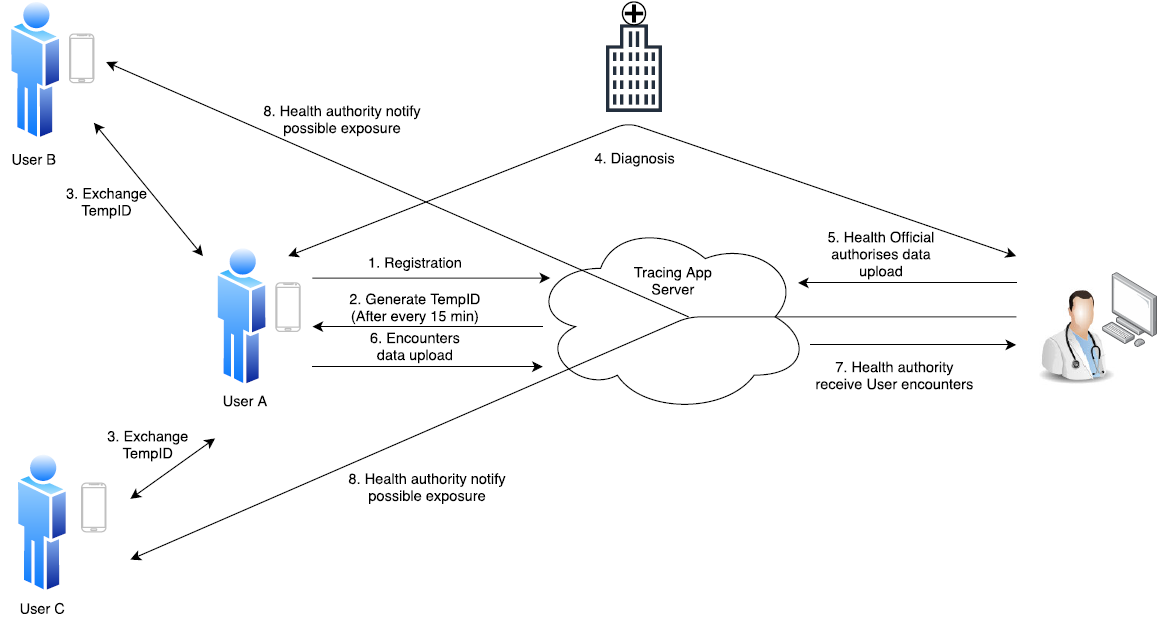
\includegraphics[width=0.8\linewidth]{images/ahmed_centralised.png}

    \caption{ Architecture Overview Diagram for Centralised Architecture from \citet{ahmed_survey_2020}.
    }

    % use the notation fig:name to cross reference a figure
    \label{fig:centralised_arch}
\end{figure}

\subsubsection{Decentralised Architecture:}

Figure \ref{fig:decentralised_arch} shows a decentralised architecture for digital contact tracing. This style of architecture performs the work on the devices, instead of performing it on a central server. The device creates and stores seeds, which are in turn used to create chirps which are short lasting pseudonyms for the device. These chirps are what is exchanged by devices and stored. When a user voluntarily uploads data only the seeds and relevant timestamps are uploaded. Other users can then download the seeds, calculate the chirps, and check if they were exposed.

Counter to the centralised architecture, the decentralised architecture having the majority of the system operations on the mobile device gives this architecture the opposite implications. The privacy is significantly better, no sign-up process is required and the main server knows very little about the users, while decreasing battery efficiency.

\begin{figure}[!htb]
    \centering
    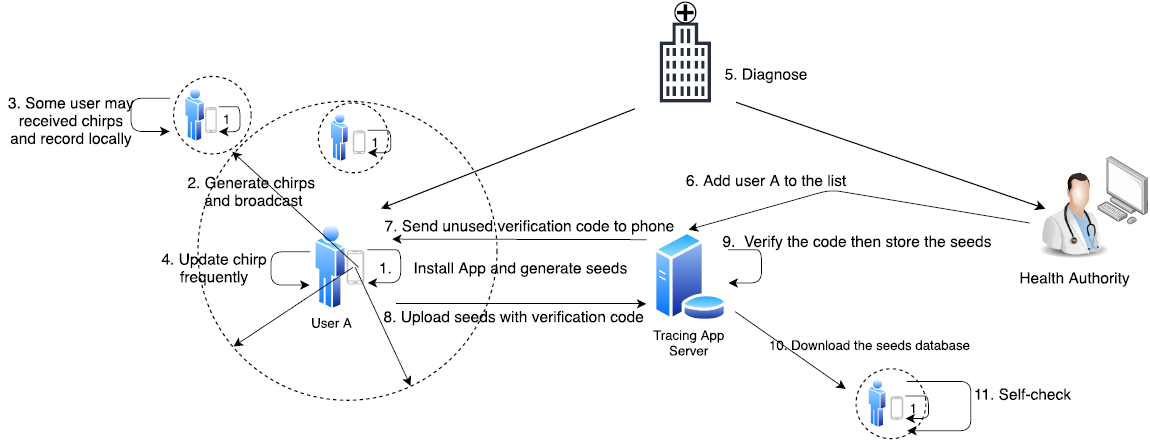
\includegraphics[width=0.8\linewidth]{images/ahmed_decentralised.png}

    \caption{ Architecture Overview Diagram for Decentralised Architecture from \citet{ahmed_survey_2020}.
    }

    % use the notation fig:name to cross reference a figure
    \label{fig:decentralised_arch}
\end{figure}

\subsubsection{Hybrid Architecture:}

The hybrid architecture, Figure \ref{fig:hybrid_arch}, the responsibilities are more evenly split between the client device and the server. Similar to the decentralised architecture the client device handles the generation of "Ephemeral IDs" which are what the devices exchange when a contact occurs. Similar to the centralised architecture the server handles calculating the risk of exposure and the notification of users who may have been exposed.

By nature of its design, the hybrid architecture is intended to compromise the benefits and drawbacks of the centralised and decentralised architecture, Having part of the process on the server allows for better identification of exposure, as it has the whole data-set to perform statistical analysis on. Also, privacy is still preserved with this architecture due to having id creation and management on device.

\begin{figure}[!htb]
    \centering
    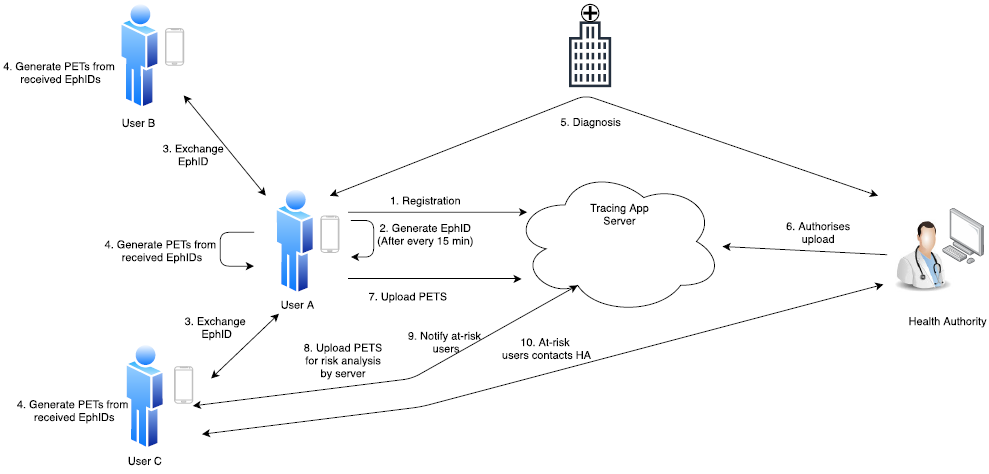
\includegraphics[width=0.8\linewidth]{images/ahmed_hybrid.png}

    \caption{ Architecture Overview Diagram for Hybrid Architecture from \citet{ahmed_survey_2020}.
    }

    % use the notation fig:name to cross reference a figure
    \label{fig:hybrid_arch}
\end{figure}

\section{Bluetooth}

\subsection{Brief Overview of Bluetooth}

Bluetooth, also referred to as Bluetooth Classic, is a wireless communications protocol, and set of specifications, designed for short-range communication between devices. Developed by the Bluetooth Special Interest Group (SIG), this technology specification has been maturing since 1999 and is currently on version 5.0 of the specification which broughy improved data transfer and tighter security. Like all wireless technologies Bluetooth operates on the electromagnetic (EM) spectrum, at a frequency of around 2.4Ghz.

\subsection{Bluetooth vs Bluetooth Low Energy}

Developed as part of the Bluetooth 4.0 specification Bluetooth Low Energy (BLE) was introduced. The primary feature in the design of BLE is its low power consumption, although this comes at the cost of having a significantly reduced throughput \citep{gomez_overview_2012}. Due to this trade-off BLE is suitable for applications that Bluetooth is not, and vice-versa, such as long-term system state monitoring solutions. Bluetooth consumes too much power, as much as 100\% more during peak power draw \citep{iot_lab_classic_2020}, to be used effectively for this.

Like Bluetooth Classic, BLE operates around the 2.4Ghz frequency band on the EM spectrum. BLE has other similarities with Bluetooth Classic, especially the lower layer architecture as seen in Figure \ref{fig:bluetooth_stack_comparison} where the controller, is very similar. They also share the Logical Link Control and Adaptation Protocol (L2CAP) layer in the host segment, which performs data translation between the upper and lower layers. This is where the similarities end.

\begin{figure}[!htb]
    \centering
    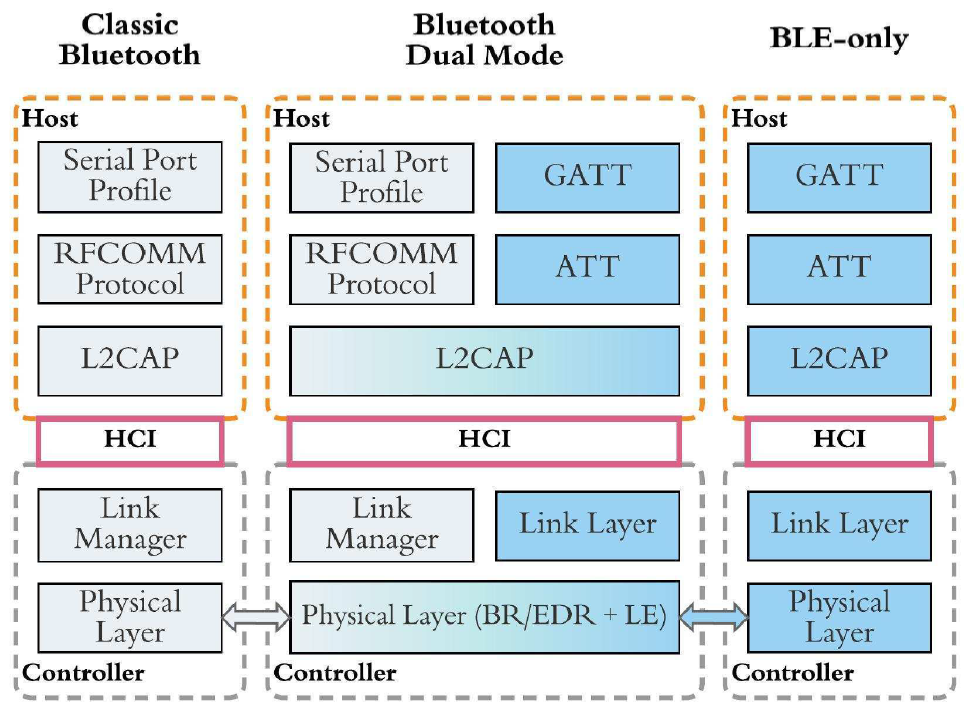
\includegraphics[width=0.8\linewidth]{images/bluetooth_stacks.png}

    \caption{ Comparative diagram of the high level Bluetooth Classic stack vs the BLE stack. The central stack is a "dual-mode" device which supports Bluetooth Classic and BLE \citep{yang_beyond_2020}. }

    % use the notation fig:name to cross reference a figure
    \label{fig:bluetooth_stack_comparison}
\end{figure}

\subsection{Bluetooth Low Energy Technical Stack - High Level}

I will give a brief overview of each layer on the BLE architecture presented in Figure \ref{fig:bluetooth_stack_comparison} from a bottom-up approach.

\subsubsection{Physical Layer:} The physical layer handles the communication hardware with a BLE system. This includes 40 radio frequency (RF) channels which, as previously stated, operate at around 2.4Ghz \citep{yang_beyond_2020}. Of these 40 channels, there are 3 dedicated advertisement channels which allow devices to detect each other and provide the necessary information for establishing a formal connection. The remaining 37 channels are used for data transmission during connections. \citet{gomez_overview_2012} states an important feature of the advertisement channels - they have been selected to mitigate against interference from common IEEE 802.11 channels, a set of standards commonly referred to as Wi-Fi.

\subsubsection{Link Layer:} This layer handles two types of communication connection-less and connection-based. \citet{yang_beyond_2020} describes that when a device only needs to send information to any devices that are listening this mechanism is used. There are two types in this scenario, the advertiser which broadcasts the information, and the scanner which is listening for these broadcasts. This happens over one of the three advertising channels, and devices can simultaneously be advertisers and scanners. Building on this, is connection-based communication. This is used when bidirectional communication is required. Here the advertisement channels are used to present a device as connectable, this is called the peripheral, then for another device to send a Connection Request, called the central \citep{gomez_overview_2012}.

\subsubsection{Host-Controller Interface:} The Host-Controller Interface (HCI) is simply a protocol layer that communicates between the host layers and the controller layers.

\subsubsection{Logical Link Control and Adaptation Protocol:} The L2CAP is held in common with Bluetooth Classic, however the BLE version is both simplified and optimised in order to meet the goals of lower power consumption. The goal is to multiplex the data of the upper layers to run along the link layer, i.e. combine the communication streams of multiple applications for simultaneous transmission \citep{gomez_overview_2012}. The L2CAP packets size is 27 bytes overall, with a 4 byte header leaving 23 bytes for the payload, shown in Figure \ref{fig:l2cap}

\begin{figure}[!htb]
    \centering
    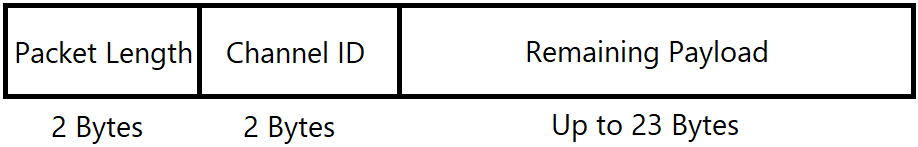
\includegraphics[width=0.8\linewidth]{images/l2cap.png}

    \caption{ Simplified packet diagram for L2CAP packets. }

    % use the notation fig:name to cross reference a figure
    \label{fig:l2cap}
\end{figure}

\subsubsection{ATT:} The attribute protocol sits atop the L2CAP layer, and manages communication between two roles, the client and the server, each of which are on separate devices. The ATT layers manages a set of attributes, this is a data structures which stores the information managed by the above layer, the GATT. An important point is that the two roles are completely separate from the central-peripheral and advertiser-scanner roles \citep{gomez_overview_2012} discussed in the link layer section above. The client can retreive, or write information from an attribute through a direct request to the server. Alternatively, the server can send the client messages in one of two types: notifications and indications. These types are the same bar the aspect where notifications don't require the client to confirm to the server it has receieved the notification. Indications do require this.

\subsubsection{GATT:} The top-level layer in the BLE stack is the genetric attribute protocol. This provides a level of abstraction over the base attributes defined in ATT, descriptors, characteristics, and services. These are linked concepts, a services is made up of characteristics, which in turn optionally contain descriptors. Descriptors provide metadata about the characteristic containing it. Characteristics are pieces of data, containing values and also properties, which act as permissions for what that characteristic allows. Finally, services are a set of related characteristics.

\subsection{Received Signal Strength Indication}

The RSSI is an indication of the reliability of the connection between two devices. \citet{SIG5.0}, in the Bluetooth 5.0 specification, describes how it can be used directly by the BLE protocol for hopping between channels, and can also be accessed by the upper layers of the BLE stack. It also states that if a device supports Received Signal Strength Indicator (RSSI) the accuracy shall be +/- 6 dB, though it should be noted that this varies between hardware implementations. Within BLE the RSSI is an absolute signal strength measurement given in decibel-milliwatts (dBm).

RSSI is commonly used in proximity estimation calculations through the use of a path loss estimation model \citep{ahmed_survey_2020}. However, there are many aspects that can affect the RSSI not just distance. These usually make the signal strength weaker. Examples are: self-interference, material based effects such as reflection and absorption, and noise from other Bluetooth signals.

\section{Background Summary}

\citet{ahmed_survey_2020} presented a survey of the current state of contact tracing as a whole. This helped highlight current methodologies and identified the current implemented methods of using Bluetooth for combatting COVID-19. This allowed for finding the commonalities between this project and existing projects, which in turn provided focus for the novel aspects. There was a heavy focus on privacy concerns; people are more likely to use something they trust. This led to a project focus of inherent privacy by design.

A core commonality between the contact tracing methods I researched, across all papers referenced in the contact tracing section, was the use of Bluetooth. This led to in-depth technical research on Bluetooth, and by extension BLE, using the core specification \citep{SIG5.0} to understand Bluetooth's viability as a distance estimating solution. \citet{gomez_overview_2012} and \citet{yang_beyond_2020} provided much needed additional context to how BLE worked in a more practical sense.

%==================================================================================================================================
\chapter{Analysis \& Requirements}

This chapter discusses the procedure for initial project analysis, and exploratory data analysis to discover specific equation parameters. From the initial analysis functional and non-functional requirements were gathered. These requirements were created in the initial phase of the project, due to how I structured the requirements there were few modifications made throughout the project lifespan.

\section{Requirements Gathering}

The process followed for requirements gathering was split into 4 artefacts, each more comprehensive than the last: A high-level mindmap, a set of user personas and stories, some user scenarios, and the requirements themselves.

\subsection{Mindmap}

The first stage of requirements gathering was the creation of a high-level mindmap. This mindmap, Figure \ref{fig:mindmap} was created to map out the initial project space; not everything contained within the mindmap made it further into the requirements gathering process.

\begin{figure}[!htb]
    \centering
    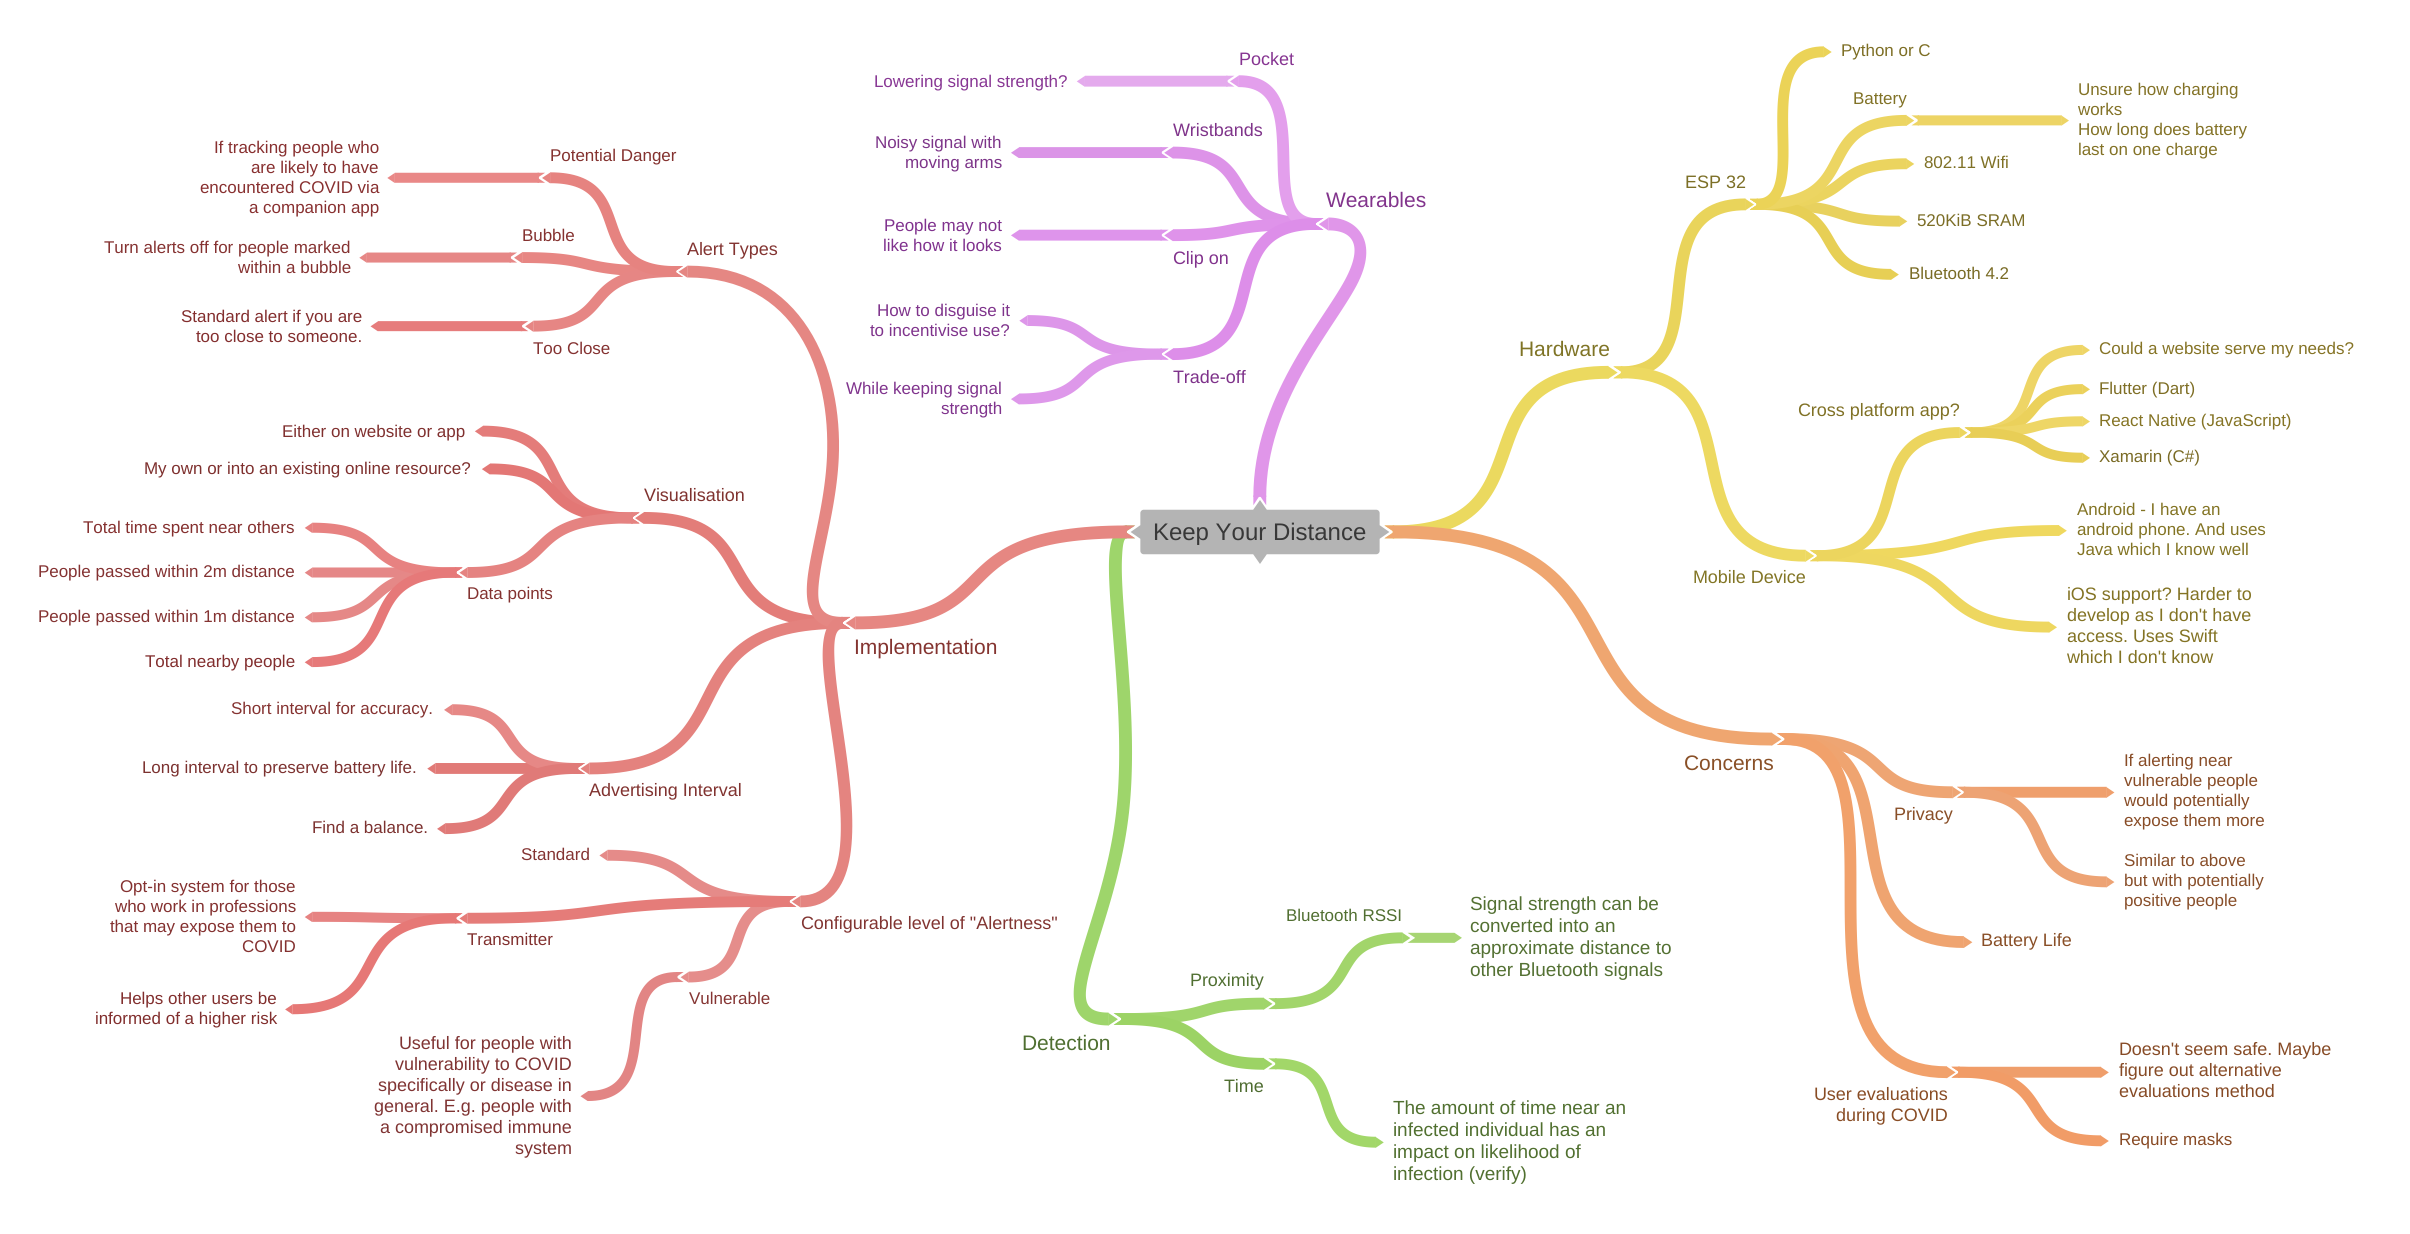
\includegraphics[width=1.0\linewidth]{images/mindmap.png}

    \caption{ High-level mindmap created as first stage of requirements gathering. }

    % use the notation fig:name to cross reference a figure
    \label{fig:mindmap}
\end{figure}

I will briefly summarise the mindmap. The mindmap is composed of five primary themes:
\begin{itemize}
    \item Implementation: Considerations to be made on potential system features such as the visualisations, or the profile system.
    \item Wearables: The initial considered set of ways to wear the device, also includes details in the trade-offs of each option.
    \item Hardware: Looking into the ESP32's hardware and the constraints I would be working with, also details technology options for the project.
    \item Concerns: Details some concerns that the system, or the project, may need to address.
    \item Detection: Examines the factors that are related to covid transmission.
\end{itemize}

\subsection{User Personas \& Stories}

User personas are fictional personalities created during requirements gathering designed to represent a user and identify user needs. User stories use these personas to provide a structured view of these needs in an "As, I want, So that" format.

Seven user personas, and related user stories, were created during requirements gathering. These covered a variety of user types, considering age, technological literacy, profession, and vulnerability to covid.

The following is an example of a user persona, and related user story:

\textbf{Alex} has a compromised immune system due to chronic illness, this puts them at a much larger degree of risk than the average person from COVID. They wish to be able to leave the house more often to have more independence but have to stay more conscious of the people around them.

As Alex, I want to keep a more strict distance from others, so that I don't become infected and become very ill.

\subsection{User Scenarios}

User scenarios utilise the user personas and stories created during the previous stage. They allow for user's wants and needs to be further examined by considering a hypothetical situation.

There was a scenario created for each story, seven in total, each scenario considers the steps the user would take to achieve some goal. For each step I considered questions I could not yet answer, ideas that the step had sparked, and general comments on how the step related to the project. For example, in Alex's Scenario (Figure \ref{fig:alex_user_scenario}), I had an idea of making the device detect people based on passive bluetooth signals but determined within the same scenario that this would be out of scope.

\section{Functional Requirements}

The set of functional requirements can be derived once the requirements gathering process had been completed. Functional requirements are actions that a user can perform on the system. These requirements were used during the development process to track criteria completion. The MoSCoW prioritisation method \citet{hudaib_requirements_2018} is common way of prioritising requirements. It works by splitting requirements into four categories, each set less important than the last. Must have (M) requirements are the minimal critical set for effective operation. Should have (S) requirements are important but not essential to system operation. Could have (C) requirements are considered nice but the system would still be usable without them. Would be nice to have (W) requirements are requirements that are considered out of scope, and will be discussed towards the end of the dissertation as future work.

\begin{itemize}
    \item \textbf{(M) Real-time RSSI Proximity Sensing: } The device must be capable of sensing another of the same device to within a 2 metre distance. It must be able to do this in near real-time.
    \item \textbf{(M) Log data to linked device for visualisation: } Since the device has no on-board storage that survives after power down there is a need to send data to device over Bluetooth connection once an interaction has occurred.
    \item \textbf{(M) Visualisations on app: } There should be visualisations and textual statistics on interaction encounters. These should be aimed at informing the user of their current habits and prompting change in necessary.
    \item \textbf{(S) Configurable device: } Allow for configuring device using pre-set profiles. This will need to be synced with the app every time the device boots as it has no power independent storage.
    \item \textbf{(S) Precision in RSSI Proximity Sensing: } The device should be capable of properly differentiating between 1 metre and 2 metre distances.
    \item \textbf{(C) Live visualisation updates on new RSSI value: } Allow for live updating graphs and statistics.
    \item \textbf{(C) Adaptive Advertising Intervals: } This is a battery consideration, a trade-off between battery consumption and advertising frequency. Would work similar on an Additive Increase system, where the interval slowly gets longer and then if it finds another device it resets back to the base interval.
    \item \textbf{(C) Organisation owned devices: } Organisations would have specific configuration tools that would allow data to be sent over Wi-Fi to their servers. The onus would be on the organisation to consider GDPR but the data from the devices would be anonymised.
    \item \textbf{(C) Battery indication on request: } Battery indicator using OLED screen but only when requested by user to preserve battery.
\end{itemize}

\section{Non-Functional Requirements}

Non-functional requirements are properties of a system which can be observed by the user. I used the same MoSCoW method the prioritise the non-functional requirements. Similar to the functional requirements, the would like to have non-functional requirements will be discussed as future work.

\begin{itemize}
    \item \textbf{(M) Colour-blind Acessibility: } The system must be usable to colour-blind users.
    \item \textbf{(M) Responsiveness: } The system must be responsive, it should not enter any waiting states.
    \item \textbf{(M) Ease of Use: } The system must be easy to use by a wide range of untrained users.
    \item \textbf{(M) App Design: } The app must follow the recommended guidance on the Android Developer Documentation.
    \item \textbf{(S) Subtle Alert: } The system should be capable of alerting the user and only the user.
    \item \textbf{(C) Organisational Privacy: } The system should not allow the organisation to identify employees from interaction information.
\end{itemize}

\section{Exploratory Data Analysis}

Exploratory data analysis was conducted both in the initial stages of the project and again later in the project with a more finished prototype. The aims of this analysis were to investigate the performance of the ESP32 BLE hardware and to find suitable parameters for calculation of the distance based on RSSI. The exact details of the formula will be discussed in the implementation section, the relevant parameters were the environment factor and the measured power.

The analysis procedure was similar in both the initial analysis and late stage analysis.  Starting from 0.5 metres apart and going up in 0.5 metre increments until 2.5 metres 250 rssi values were recorded. The NumPy and Pandas python libraries were used for data processsing, along with MatplotLib and Seaborn being used for data visualisation. A large range of graphs were created including violinplots, swarmplots, histograms, density plots, and line graphs.

The violinplot of RSSI values against specific distances (0.5m - 2.5m) were useful in getting a high level comparative overview on how the RSSI values were clustered, along with how they varied. To allow for easier comparison a density estimation plot was created which allowed for much easier identification of distinct areas along with overlapping areas that may be problematic.

For finding the best parameters a separate dataset was computed for each environment variable value (integers 1 through 4), considering 50 RSSI values from -100 to -50. For each RSSI value the estimated distance was calculated. These datasets were then compared to the real dataset to find the best fit for each environment variable. To then find the best environment variable the standard deviation of the error between the real dataset and each theoretical dataset was calculated. To show this visually a series of linecharts were created to show the error for each distance category, the mean error, and the median error.

\subsection{Initial Analysis}

For the initial analysis data collection the early prototype version didn't have any form of timing system to determine when packets were missed so as workaround I had the receiving device listen every second, and record a dummy value if a packet wasn't received. This initial analysis was particularly important as it showed the project had potential using the ESP32 hardware Figure \ref{fig:initial_density}. A best parameter fit of environment = 3, measure power = -81 was identified as shown in \ref{fig:initial_best_fit}.

\begin{figure}[!htb]
    \centering
    \begin{subfigure}[b]{0.45\textwidth}
        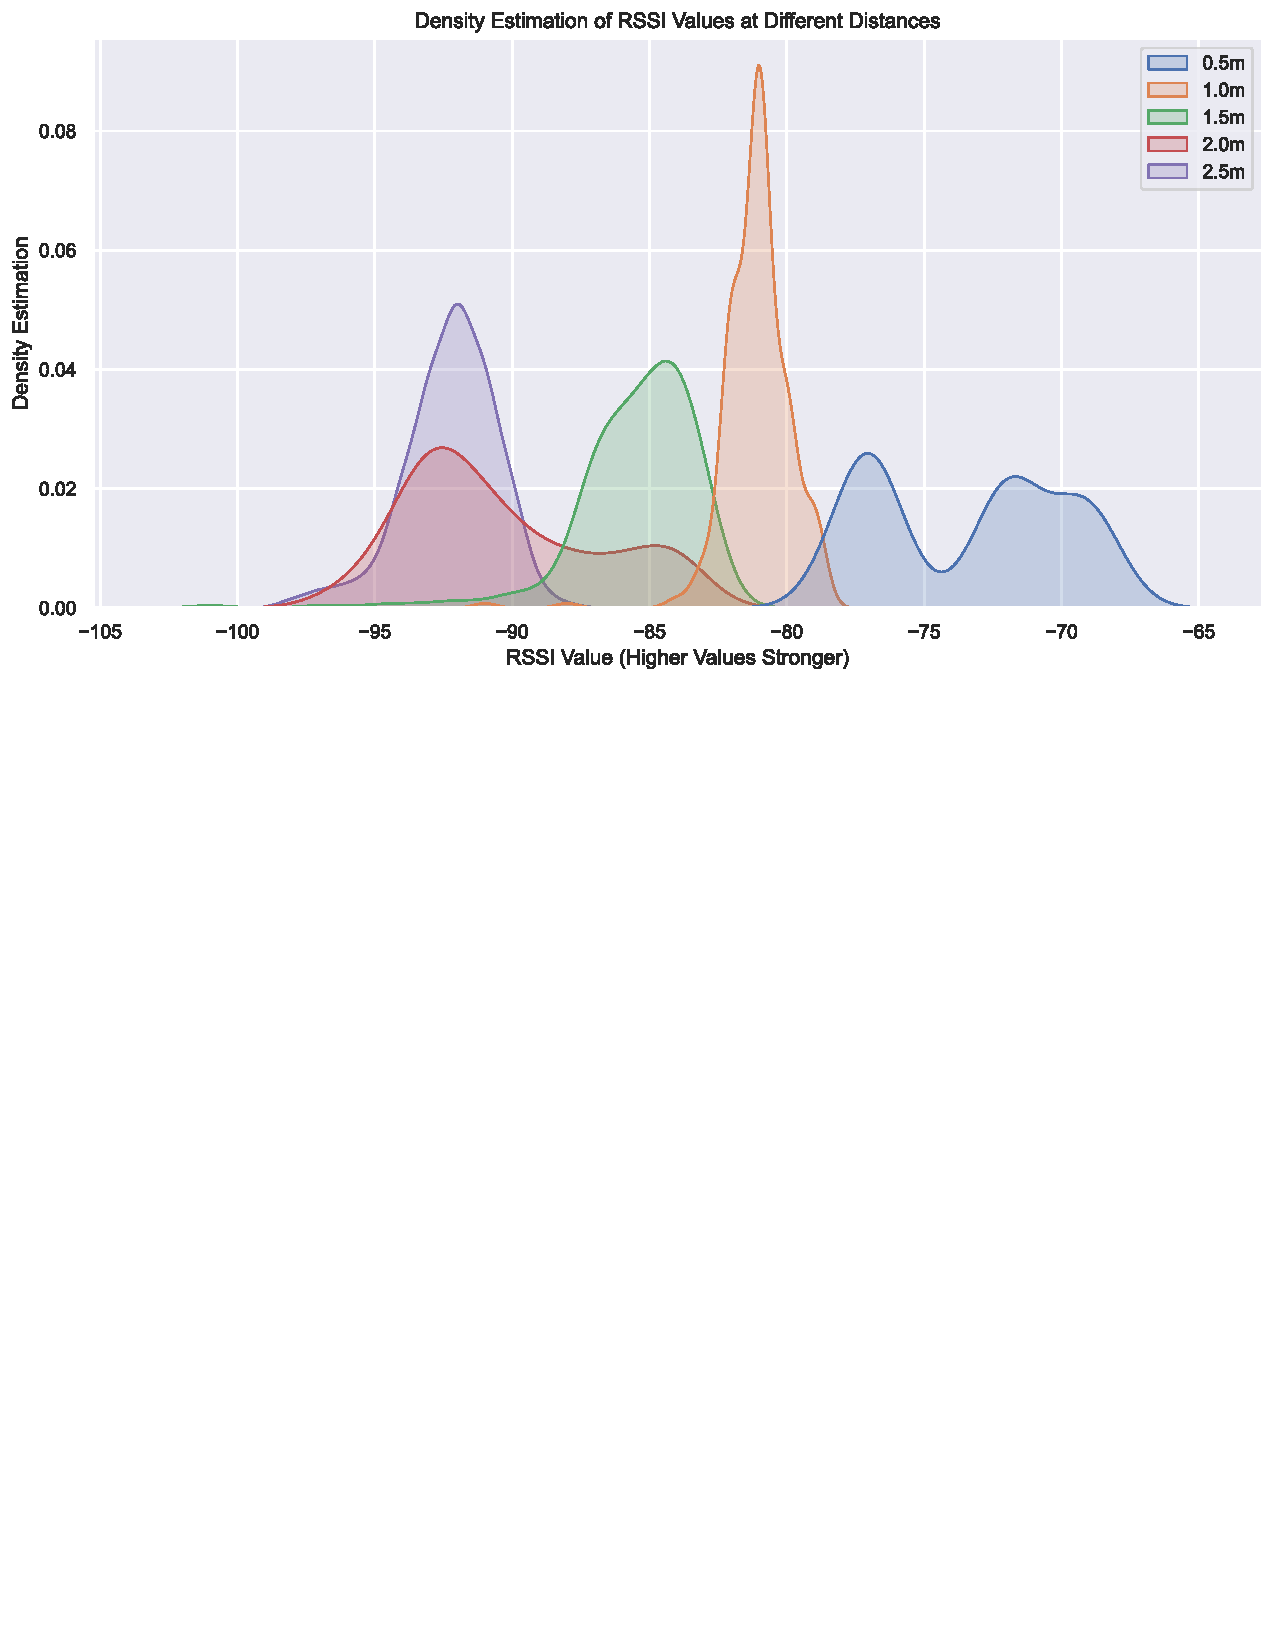
\includegraphics[width=\textwidth]{images/initial_rssi_density.pdf}
        \caption{Density estimation plot for initial exploratory data analysis. Note the distinct peaks for most distances with the exception of red (2.0m) and purple (2.5m).}
        \label{fig:initial_density}
    \end{subfigure}
    ~
    \begin{subfigure}[b]{0.45\textwidth}
        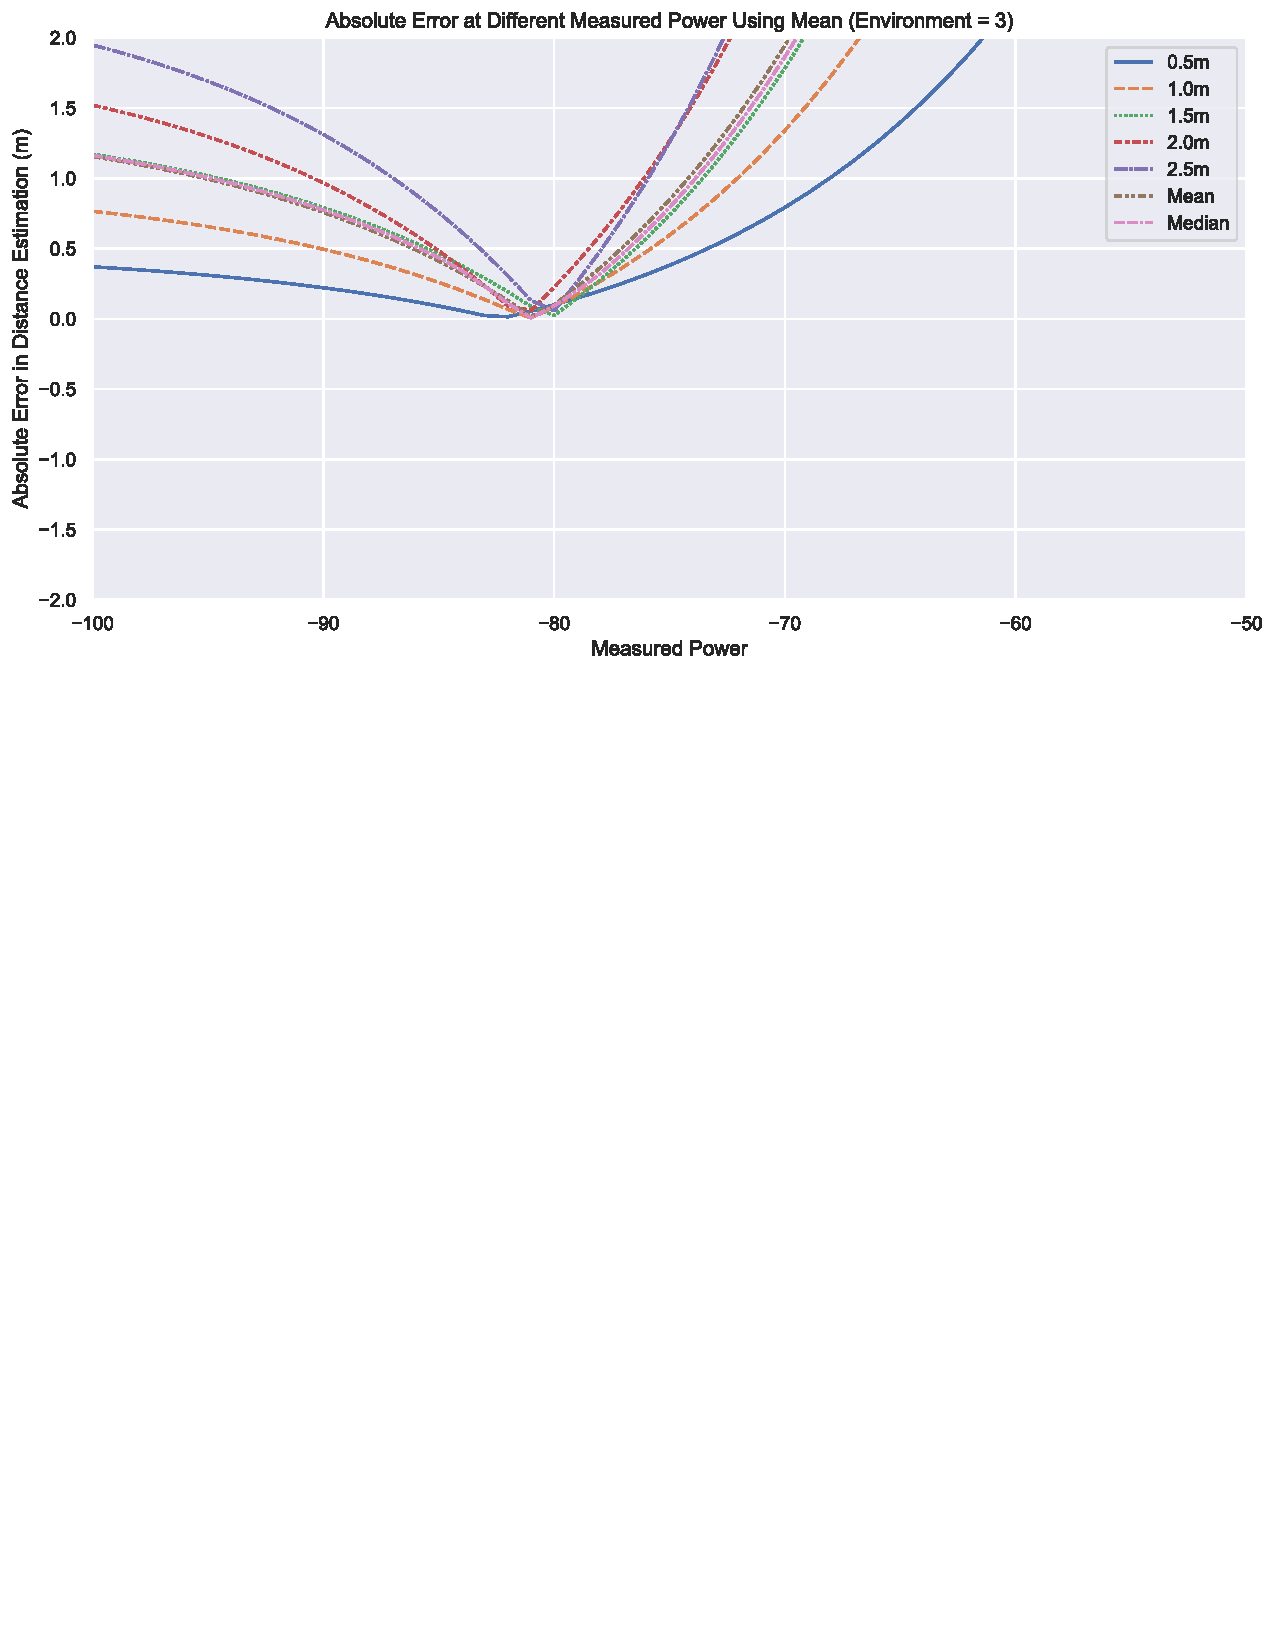
\includegraphics[width=\textwidth]{images/initial_mp_bestfit.pdf}
        \caption{Best fit error plot for initial exploratory data analysis. Graph for environment = 3, shows most common point when measured power = -81.}
        \label{fig:initial_best_fit}
    \end{subfigure}
    ~ %add desired spacing between images, e. g. ~, \quad, \qquad, \hfill etc. 
    %(or a blank line to force the subfigure onto a new line)    
    \caption{ Key plots from initial exploratory data analysis. }
    \label{fig:density_plots}
\end{figure}

\subsection{Late Stage Analysis}

In the late stage analysis the timing system was fully implemented so I could determine packet loss between packets received. Two types of areas were covered in the late stage analysis: Indoor, and Urban Outdoor. Originally a Remote Outdoor investigation was planned however this was not feasible to set up. For each area the devices were set up in three ways: facing pin side up, facing pin side down, and hanging mid-air facing each other. The aim of this analysis was similar to the initial analysis but with more of a focus on determining real world performance as opposed to technical feasibility.

After conducting the pin side up and pin side down versions of the indoor experiment and analysing the results , the densities of the distances seemed to have a large amount of overlap Figure \ref{fig:indoor_up_density} - much more than expected, and much more than the initial analysis. I then decided to run the experiment again but with a new setup, I had the ESP32s hanging off opposing faces. This allowed for a more realistic scenario as the devices would be facing each other as they would be when worn on people. This yielded closer to the expected result, Figure \ref{fig:indoor_hanging_density}. There was still overlap, however it was clustered into sections. These clusters were 0.5m, 1.0m \& 1.5m, and 2.0m \& 2.5m. Ideally each distance would be separately indentifiable as was the case with the initial analysis, however this is still a positive result as it does allow for distinct distance identification.

\begin{figure}[!htb]
    \centering
    \begin{subfigure}[b]{0.45\textwidth}
        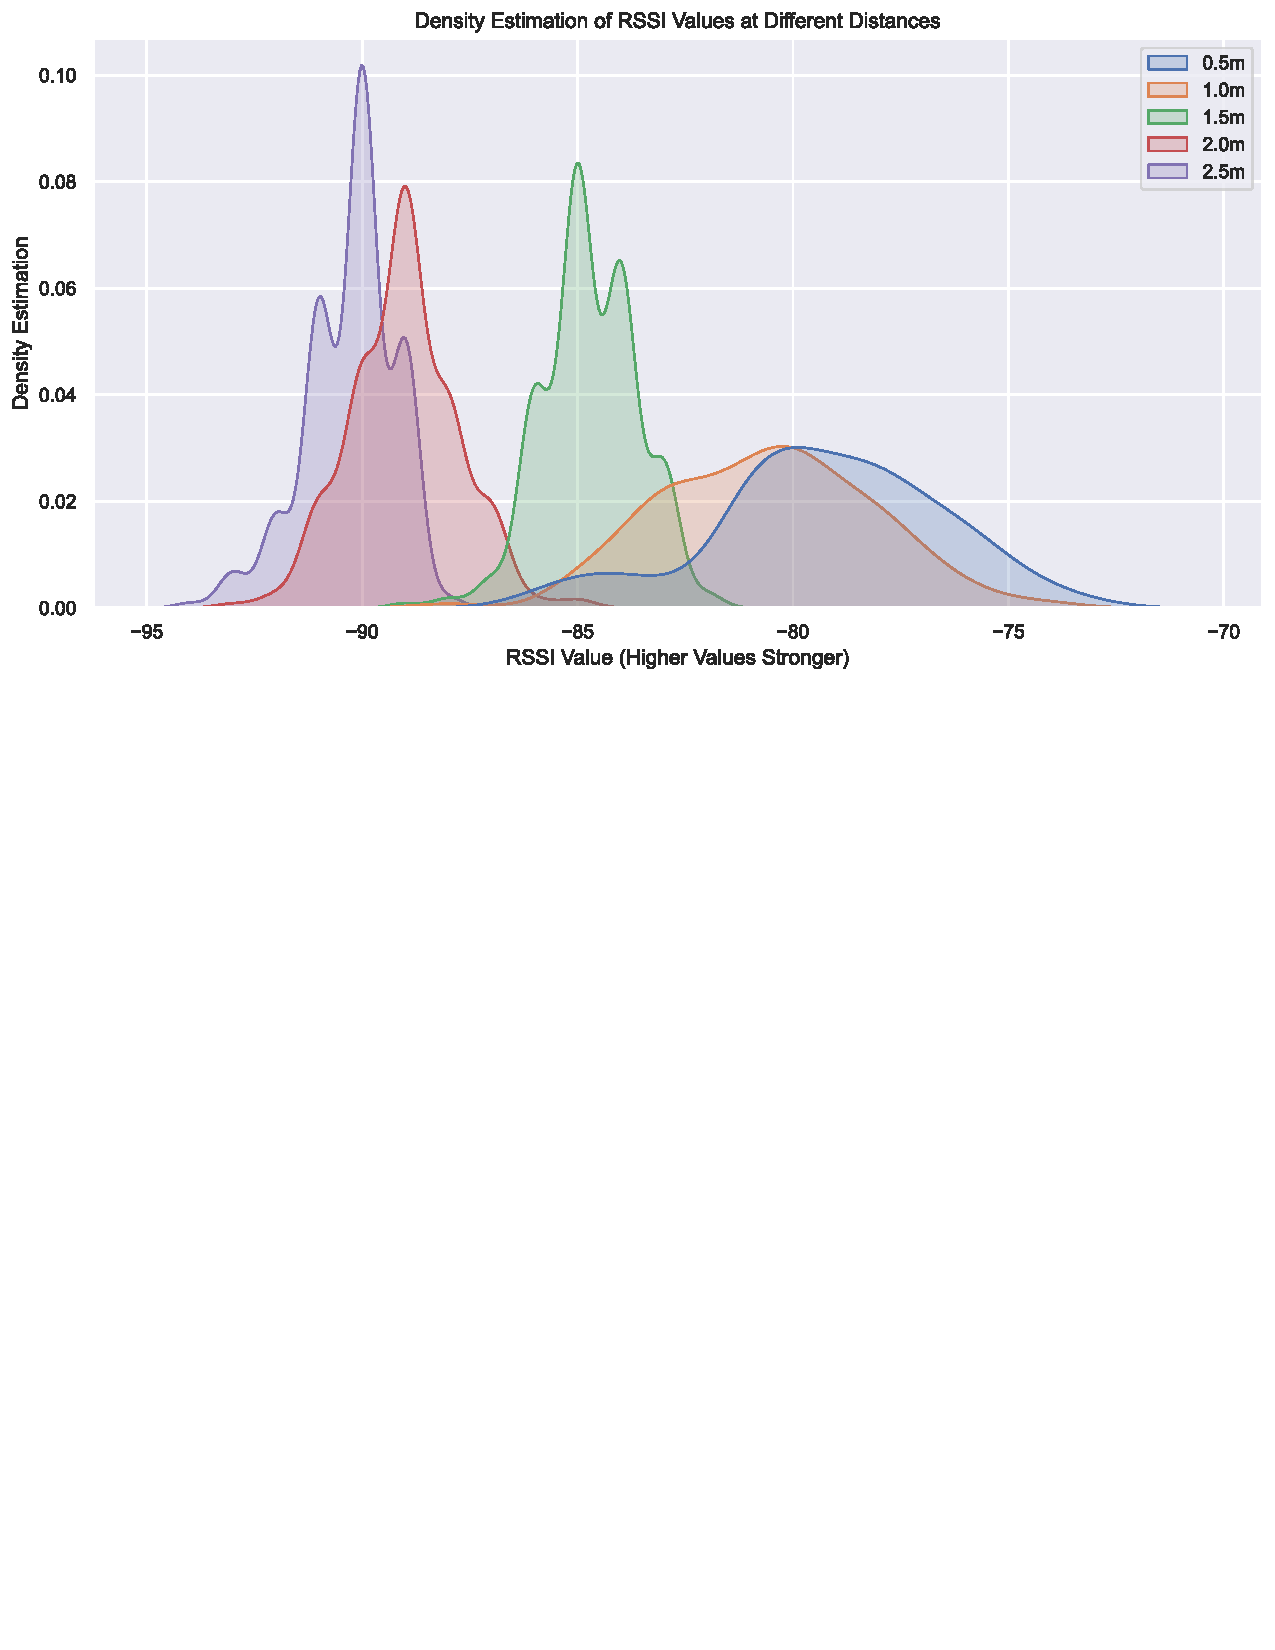
\includegraphics[width=\textwidth]{images/indoor_up_rssi_density.pdf}
        \caption{ Density estimation plot for the indoor pin side up experiment.  }
        \label{fig:indoor_up_density}
    \end{subfigure}
    ~
    \begin{subfigure}[b]{0.45\textwidth}
        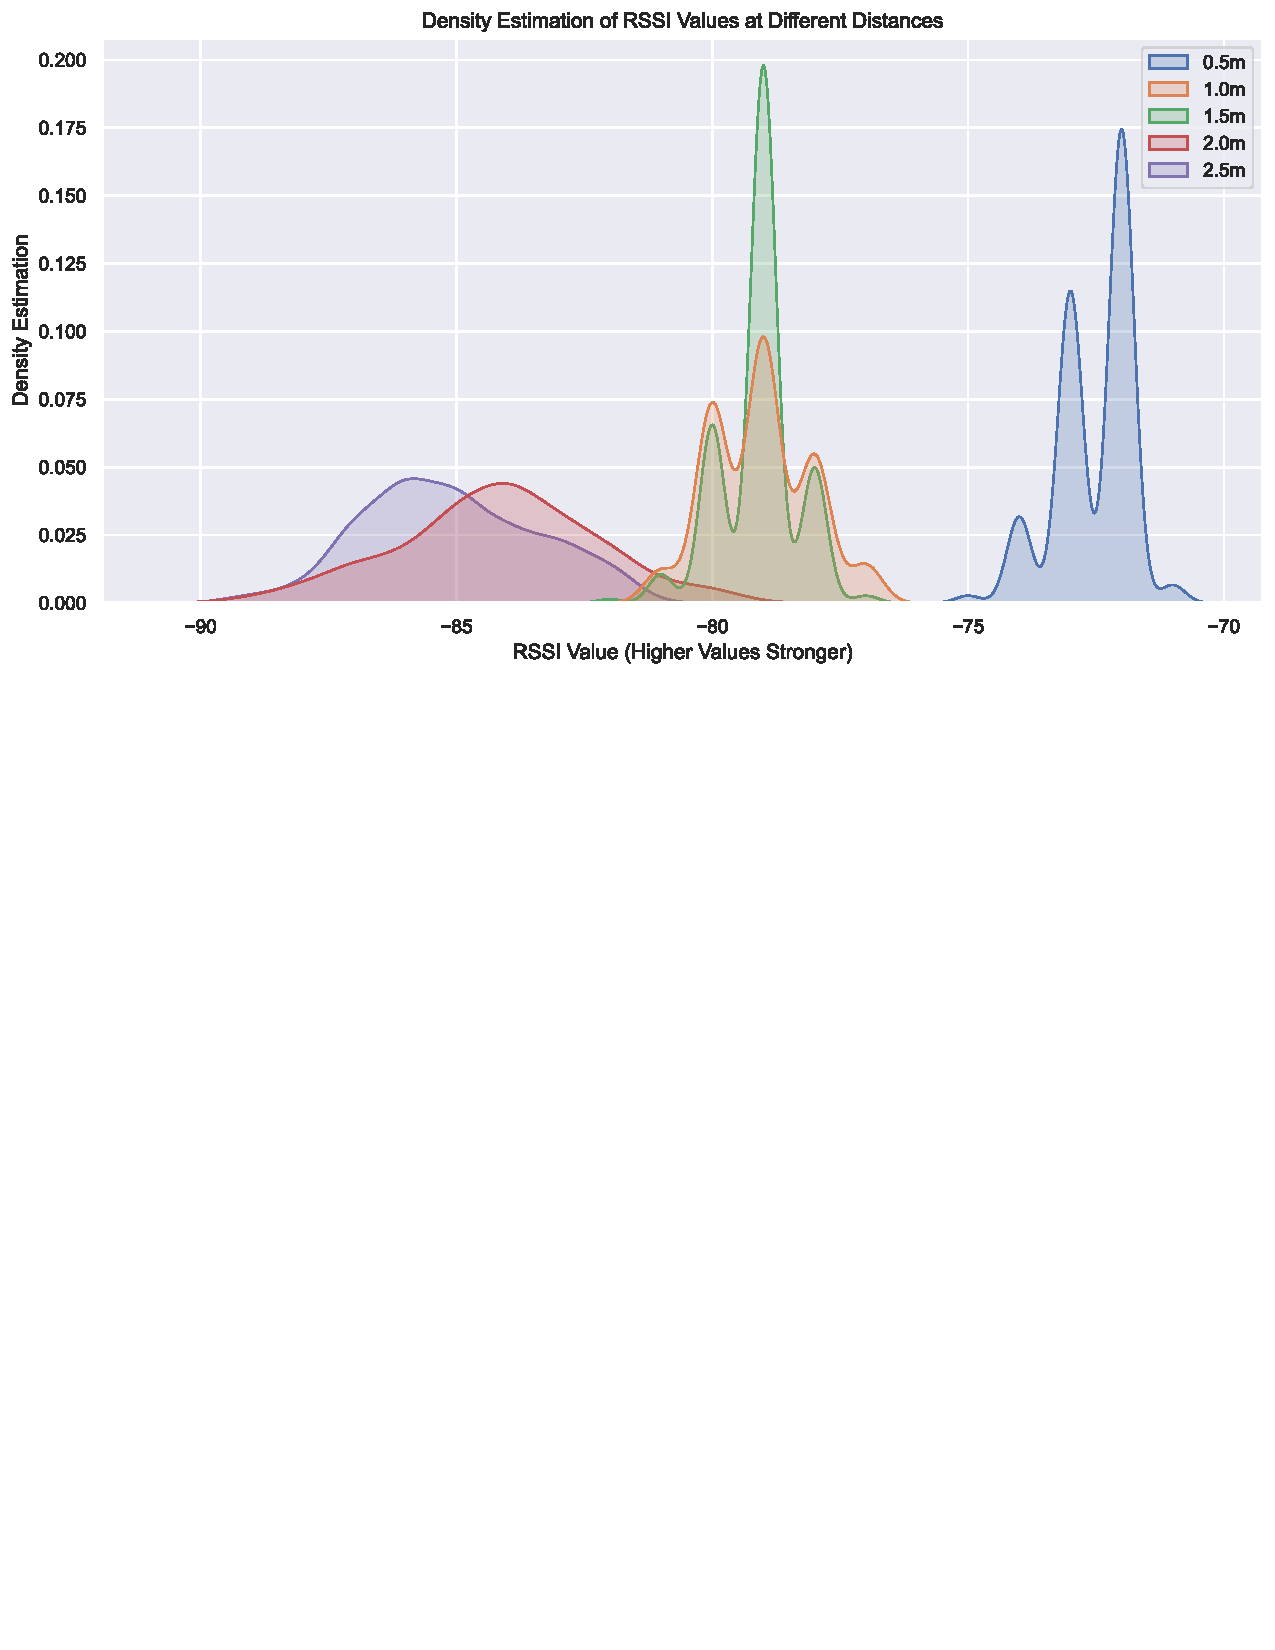
\includegraphics[width=\textwidth]{images/indoor_hanging_rssi_density.pdf}
        \caption{ Density estimation plot for the indoor hanging experiment. }
        \label{fig:indoor_hanging_density}
    \end{subfigure}
    ~ %add desired spacing between images, e. g. ~, \quad, \qquad, \hfill etc. 
    %(or a blank line to force the subfigure onto a new line)    
    \caption{ Comparison of the pin side up experiment density \subref{fig:indoor_up_density} vs the hanging experiment density\subref{fig:indoor_hanging_density} for indoors. The hanging experiment creates more identifiable clusters. }
    \label{fig:initial_plots}
\end{figure}

To ensure fairness between experiments all three variants of the experiment were performed when doing the outdoor experiment. As expected this yielded similar results to the indoor experiment though with somewhat better clustering overall. However, a key drawback to the outdoor conditions was more difficulty in receiving a signal between the two devices; the pin side up variation was unable to get a consistent connection at 2.5 metres. This can be explained when considering the surrounding surfaces. Since waves are reflected off of surfaces, when indoors there is more surface area to bounce off and reach the other device.

Since the hanging variant of the experiments is the most realistic in terms of mimicking real world device use these dataset were used to calculate best fit parameters for the Indoor and Outdoor City profiles. The resulting parameters were very similar with the Indoor, Figure  having parameters environment = 2, measured power = -78, Figure \ref{fig:indoor_hanging_bestfit}; Outdoor City was calculated to have the same environment and a measured power of -78, Figure \ref{fig:outdoor_hanging_bestfit}.

\begin{figure}[!htb]
    \centering
    \begin{subfigure}[b]{0.45\textwidth}
        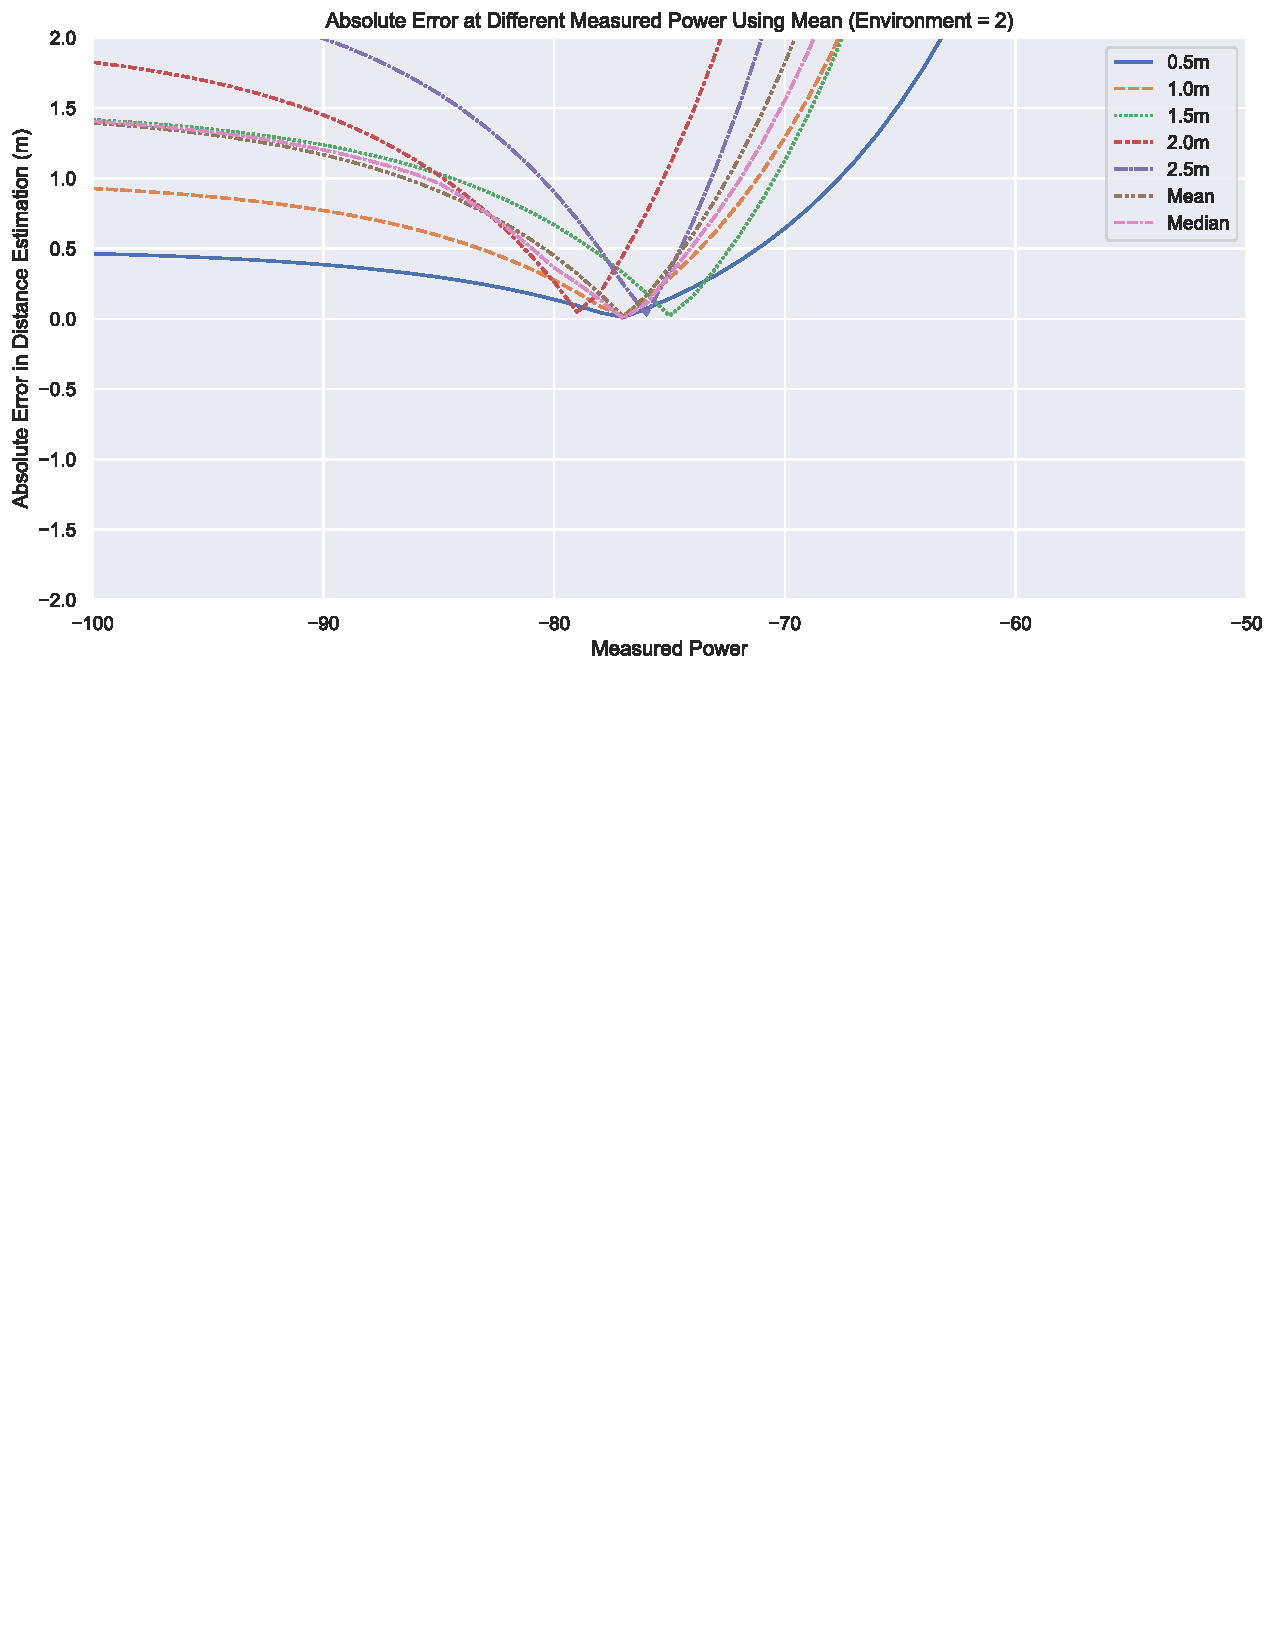
\includegraphics[width=\textwidth]{images/indoor_hanging_bestfit.pdf}
        \caption{ Best-fit graph for the indoor experiment. }
        \label{fig:indoor_hanging_bestfit}
    \end{subfigure}
    ~
    \begin{subfigure}[b]{0.45\textwidth}
        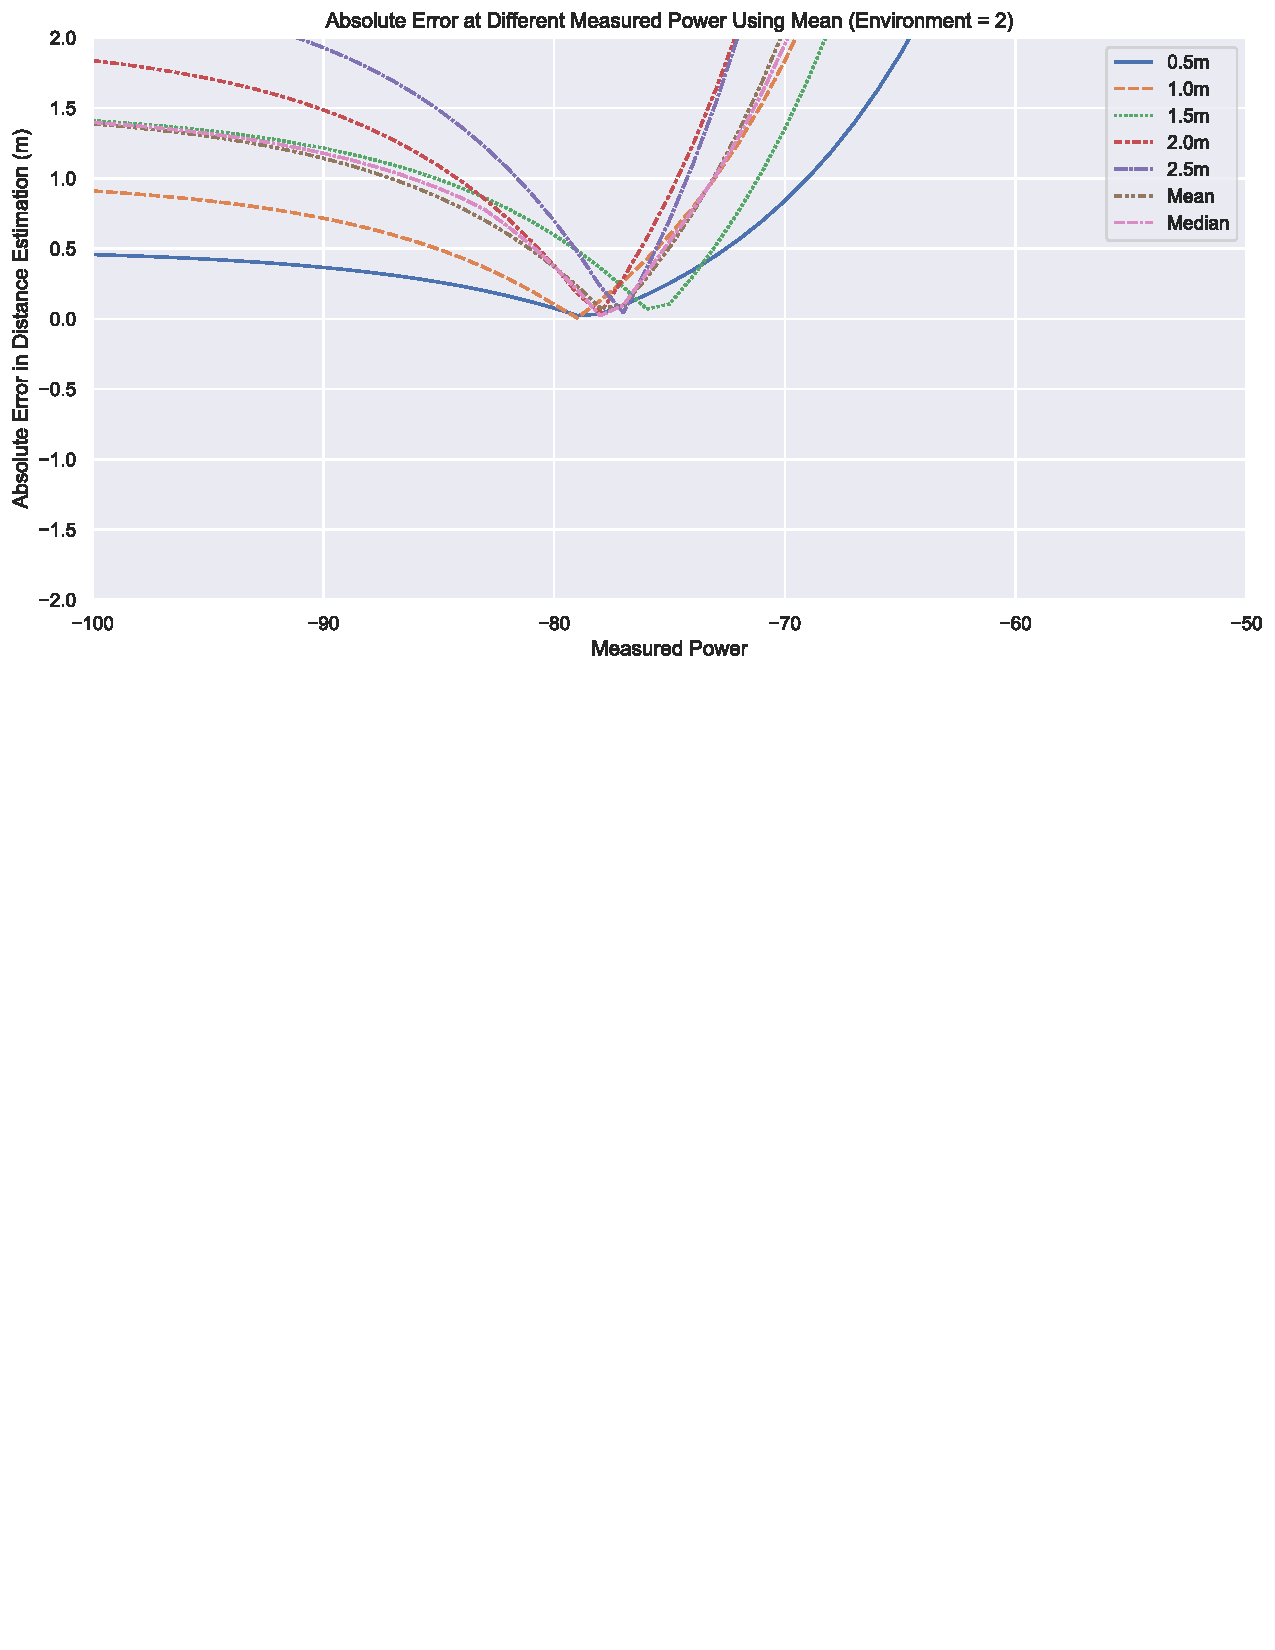
\includegraphics[width=\textwidth]{images/outdoor_hanging_bestfit.pdf}
        \caption{ Best-fit graph for the outdoor experiment. }
        \label{fig:outdoor_hanging_bestfit}
    \end{subfigure}
    ~ %add desired spacing between images, e. g. ~, \quad, \qquad, \hfill etc. 
    %(or a blank line to force the subfigure onto a new line)    
    \caption{ Best-fit graphs based off the hanging experiment variants. }
    \label{fig:bestfit_plots}
\end{figure}

\subsection{Requirements \& Analysis Summary}

The section discussed the requirements gathering process that was used during this project. The MoSCoW prioritisation method was used to allow for a strong set of requirements that had the flexibility to accomodate project changes without having to modify the requirements list. It also discussed how parameter values were identified that could be used during the design and implementation stages.

%==================================================================================================================================
\chapter{Design}
How is this problem to be approached, without reference to specific implementation details?
\section{Guidance}
Design should cover the abstract design in such a way that someone else might be able to do what you did, but with a different language or library or tool.

%==================================================================================================================================
\chapter{Implementation}
What did you do to implement this idea, and what technical achievements did you make?

\section{ESP 32}

\textbf{Short section on the esp32 to introduce it - maybe better for design section - ask Jeremy his opinion on this. }\\

\section{Guidance}
You can't talk about everything. Cover the high level first, then cover important, relevant or impressive details.



\section{General points}

These points apply to the whole dissertation, not just this chapter.



\subsection{Figures}
\emph{Always} refer to figures included, like Figure \ref{fig:relu}, in the body of the text. Include full, explanatory captions and make sure the figures look good on the page.
You may include multiple figures in one float, as in Figure \ref{fig:synthetic}, using \texttt{subcaption}, which is enabled in the template.



% Figures are important. Use them well.
\begin{figure}
    \centering
    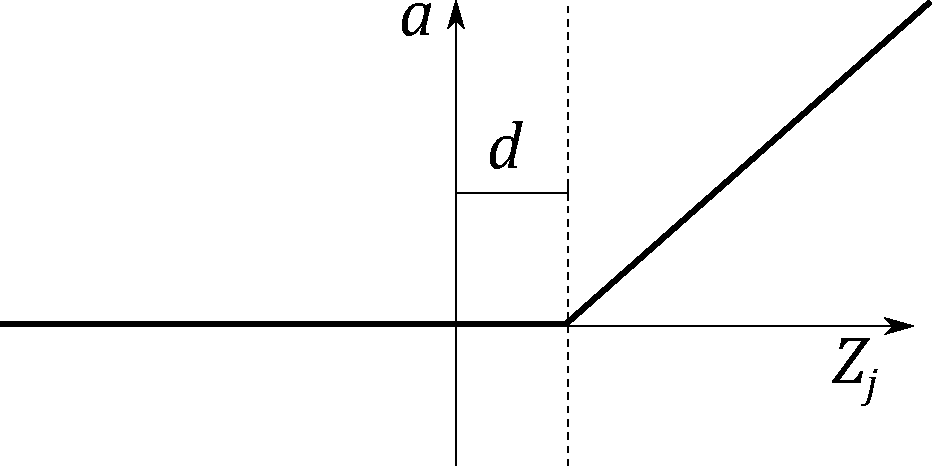
\includegraphics[width=0.5\linewidth]{images/relu.pdf}

    \caption{In figure captions, explain what the reader is looking at: ``A schematic of the rectifying linear unit, where $a$ is the output amplitude,
        $d$ is a configurable dead-zone, and $Z_j$ is the input signal'', as well as why the reader is looking at this:
        ``It is notable that there is no activation \emph{at all} below 0, which explains our initial results.''
        \textbf{Use vector image formats (.pdf) where possible}. Size figures appropriately, and do not make them over-large or too small to read.
    }

    % use the notation fig:name to cross reference a figure
    \label{fig:relu}
\end{figure}


\begin{figure}
    \centering
    \begin{subfigure}[b]{0.45\textwidth}
        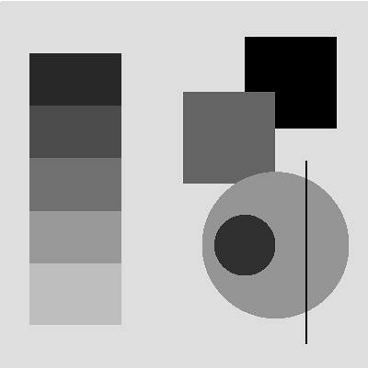
\includegraphics[width=\textwidth]{images/synthetic.png}
        \caption{Synthetic image, black on white.}
        \label{fig:syn1}
    \end{subfigure}
    ~ %add desired spacing between images, e. g. ~, \quad, \qquad, \hfill etc. 
    %(or a blank line to force the subfigure onto a new line)
    \begin{subfigure}[b]{0.45\textwidth}
        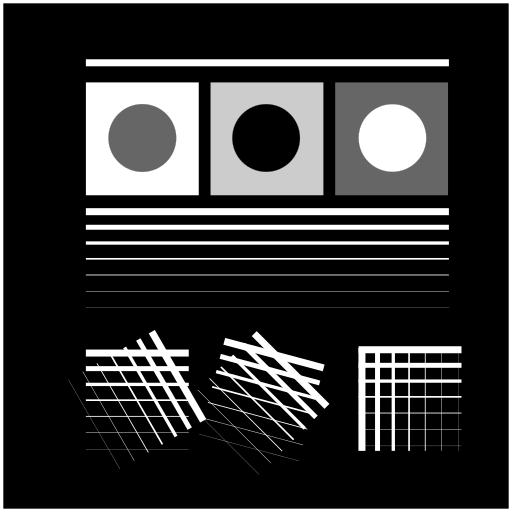
\includegraphics[width=\textwidth]{images/synthetic_2.png}
        \caption{Synthetic image, white on black.}
        \label{fig:syn2}
    \end{subfigure}
    ~ %add desired spacing between images, e. g. ~, \quad, \qquad, \hfill etc. 
    %(or a blank line to force the subfigure onto a new line)    
    \caption{Synthetic test images for edge detection algorithms. \subref{fig:syn1} shows various gray levels that require an adaptive algorithm. \subref{fig:syn2}
        shows more challenging edge detection tests that have crossing lines. Fusing these into full segments typically requires algorithms like the Hough transform.
        This is an example of using subfigures, with \texttt{subref}s in the caption.
    }\label{fig:synthetic}
\end{figure}

\clearpage

\subsection{Equations}

Equations should be typeset correctly and precisely. Make sure you get parenthesis sizing correct, and punctuate equations correctly
(the comma is important and goes \textit{inside} the equation block). Explain any symbols used clearly if not defined earlier.

For example, we might define:
\begin{equation}
    \hat{f}(\xi) = \frac{1}{2}\left[ \int_{-\infty}^{\infty} f(x) e^{2\pi i x \xi} \right],
\end{equation}
where $\hat{f}(\xi)$ is the Fourier transform of the time domain signal $f(x)$.

\subsection{Algorithms}
Algorithms can be set using \texttt{algorithm2e}, as in Algorithm \ref{alg:metropolis}.

% NOTE: line ends are denoted by \; in algorithm2e
\begin{algorithm}
    \DontPrintSemicolon
    \KwData{$f_X(x)$, a probability density function returing the density at $x$.\; $\sigma$ a standard deviation specifying the spread of the proposal distribution.\;
        $x_0$, an initial starting condition.}
    \KwResult{$s=[x_1, x_2, \dots, x_n]$, $n$ samples approximately drawn from a distribution with PDF $f_X(x)$.}
    \Begin{
        $s \longleftarrow []$\;
        $p \longleftarrow f_X(x)$\;
        $i \longleftarrow 0$\;
        \While{$i < n$}
        {
            $x^\prime \longleftarrow \mathcal{N}(x, \sigma^2)$\;
            $p^\prime \longleftarrow f_X(x^\prime)$\;
            $a \longleftarrow \frac{p^\prime}{p}$\;
            $r \longleftarrow U(0,1)$\;
            \If{$r<a$}
            {
                $x \longleftarrow x^\prime$\;
                $p \longleftarrow f_X(x)$\;
                $i \longleftarrow i+1$\;
                append $x$ to $s$\;
            }
        }
    }

    \caption{The Metropolis-Hastings MCMC algorithm for drawing samples from arbitrary probability distributions,
        specialised for normal proposal distributions $q(x^\prime|x) = \mathcal{N}(x, \sigma^2)$. The symmetry of the normal distribution means the acceptance rule takes the simplified form.}\label{alg:metropolis}
\end{algorithm}

\subsection{Tables}

If you need to include tables, like Table \ref{tab:operators}, use a tool like https://www.tablesgenerator.com/ to generate the table as it is
extremely tedious otherwise.

\begin{table}[]
    \caption{The standard table of operators in Python, along with their functional equivalents from the \texttt{operator} package. Note that table
        captions go above the table, not below. Do not add additional rules/lines to tables. }\label{tab:operators}
    %\tt 
    \rowcolors{2}{}{gray!3}
    \begin{tabular}{@{}lll@{}}
        %\toprule
        \textbf{Operation}    & \textbf{Syntax}                         & \textbf{Function}                          \\ %\midrule % optional rule for header
        Addition              & \texttt{a + b}                          & \texttt{add(a, b)}                         \\
        Concatenation         & \texttt{seq1 + seq2}                    & \texttt{concat(seq1, seq2)}                \\
        Containment Test      & \texttt{obj in seq}                     & \texttt{contains(seq, obj)}                \\
        Division              & \texttt{a / b}                          & \texttt{div(a, b) }                        \\
        Division              & \texttt{a / b}                          & \texttt{truediv(a, b) }                    \\
        Division              & \texttt{a // b}                         & \texttt{floordiv(a, b)}                    \\
        Bitwise And           & \texttt{a \& b}                         & \texttt{and\_(a, b)}                       \\
        Bitwise Exclusive Or  & \texttt{a \textasciicircum b}           & \texttt{xor(a, b)}                         \\
        Bitwise Inversion     & \texttt{$\sim$a}                        & \texttt{invert(a)}                         \\
        Bitwise Or            & \texttt{a | b}                          & \texttt{or\_(a, b)}                        \\
        Exponentiation        & \texttt{a ** b}                         & \texttt{pow(a, b)}                         \\
        Identity              & \texttt{a is b}                         & \texttt{is\_(a, b)}                        \\
        Identity              & \texttt{a is not b}                     & \texttt{is\_not(a, b)}                     \\
        Indexed Assignment    & \texttt{obj{[}k{]} = v}                 & \texttt{setitem(obj, k, v)}                \\
        Indexed Deletion      & \texttt{del obj{[}k{]}}                 & \texttt{delitem(obj, k)}                   \\
        Indexing              & \texttt{obj{[}k{]}}                     & \texttt{getitem(obj, k)}                   \\
        Left Shift            & \texttt{a \textless{}\textless b}       & \texttt{lshift(a, b)}                      \\
        Modulo                & \texttt{a \% b}                         & \texttt{mod(a, b)}                         \\
        Multiplication        & \texttt{a * b}                          & \texttt{mul(a, b)}                         \\
        Negation (Arithmetic) & \texttt{- a}                            & \texttt{neg(a)}                            \\
        Negation (Logical)    & \texttt{not a}                          & \texttt{not\_(a)}                          \\
        Positive              & \texttt{+ a}                            & \texttt{pos(a)}                            \\
        Right Shift           & \texttt{a \textgreater{}\textgreater b} & \texttt{rshift(a, b)}                      \\
        Sequence Repetition   & \texttt{seq * i}                        & \texttt{repeat(seq, i)}                    \\
        Slice Assignment      & \texttt{seq{[}i:j{]} = values}          & \texttt{setitem(seq, slice(i, j), values)} \\
        Slice Deletion        & \texttt{del seq{[}i:j{]}}               & \texttt{delitem(seq, slice(i, j))}         \\
        Slicing               & \texttt{seq{[}i:j{]}}                   & \texttt{getitem(seq, slice(i, j))}         \\
        String Formatting     & \texttt{s \% obj}                       & \texttt{mod(s, obj)}                       \\
        Subtraction           & \texttt{a - b}                          & \texttt{sub(a, b)}                         \\
        Truth Test            & \texttt{obj}                            & \texttt{truth(obj)}                        \\
        Ordering              & \texttt{a \textless b}                  & \texttt{lt(a, b)}                          \\
        Ordering              & \texttt{a \textless{}= b}               & \texttt{le(a, b)}                          \\
        % \bottomrule
    \end{tabular}
\end{table}
\subsection{Code}

Avoid putting large blocks of code in the report (more than a page in one block, for example). Use syntax highlighting if possible, as in Listing \ref{lst:callahan}.

\begin{lstlisting}[language=python, float, caption={The algorithm for packing the $3\times 3$ outer-totalistic binary CA successor rule into a 
    $16\times 16\times 16\times 16$ 4 bit lookup table, running an equivalent, notionally 16-state $2\times 2$ CA.}, label=lst:callahan]
    def create_callahan_table(rule="b3s23"):
        """Generate the lookup table for the cells."""        
        s_table = np.zeros((16, 16, 16, 16), dtype=np.uint8)
        birth, survive = parse_rule(rule)

        # generate all 16 bit strings
        for iv in range(65536):
            bv = [(iv >> z) & 1 for z in range(16)]
            a, b, c, d, e, f, g, h, i, j, k, l, m, n, o, p = bv

            # compute next state of the inner 2x2
            nw = apply_rule(f, a, b, c, e, g, i, j, k)
            ne = apply_rule(g, b, c, d, f, h, j, k, l)
            sw = apply_rule(j, e, f, g, i, k, m, n, o)
            se = apply_rule(k, f, g, h, j, l, n, o, p)

            # compute the index of this 4x4
            nw_code = a | (b << 1) | (e << 2) | (f << 3)
            ne_code = c | (d << 1) | (g << 2) | (h << 3)
            sw_code = i | (j << 1) | (m << 2) | (n << 3)
            se_code = k | (l << 1) | (o << 2) | (p << 3)

            # compute the state for the 2x2
            next_code = nw | (ne << 1) | (sw << 2) | (se << 3)

            # get the 4x4 index, and write into the table
            s_table[nw_code, ne_code, sw_code, se_code] = next_code

        return s_table

\end{lstlisting}

%==================================================================================================================================
\chapter{Evaluation}
How good is your solution? How well did you solve the general problem, and what evidence do you have to support that?

\section{Guidance}
\begin{itemize}
    \item
          Ask specific questions that address the general problem.
    \item
          Answer them with precise evidence (graphs, numbers, statistical
          analysis, qualitative analysis).
    \item
          Be fair and be scientific.
    \item
          The key thing is to show that you know how to evaluate your work, not
          that your work is the most amazing product ever.
\end{itemize}

\section{Evidence}
Make sure you present your evidence well. Use appropriate visualisations, reporting techniques and statistical analysis, as appropriate.

If you visualise, follow the basic rules, as illustrated in Figure \ref{fig:boxplot}:
\begin{itemize}
    \item Label everything correctly (axis, title, units).
    \item Caption thoroughly.
    \item Reference in text.
    \item \textbf{Include appropriate display of uncertainty (e.g. error bars, Box plot)}
    \item Minimize clutter.
\end{itemize}

See the file \texttt{guide\_to\_visualising.pdf} for further information and guidance.

\begin{figure}
    \centering
    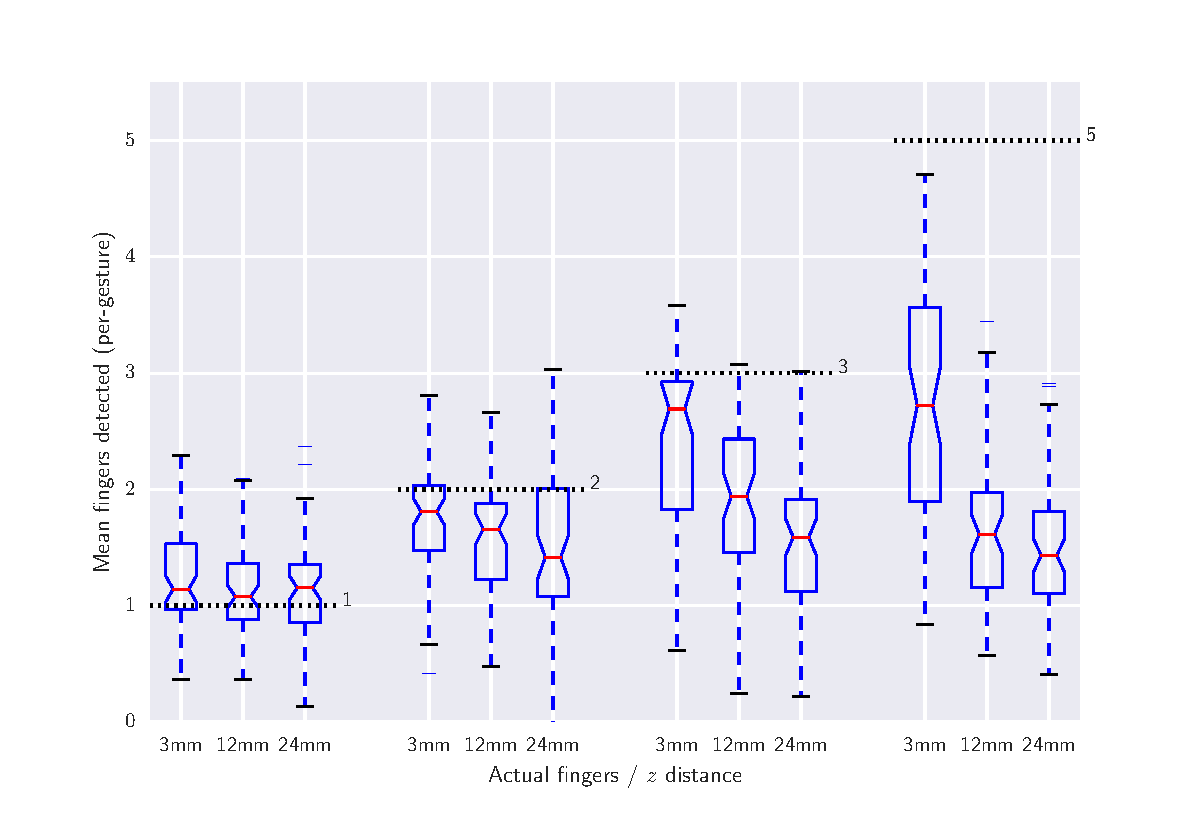
\includegraphics[width=1.0\linewidth]{images/boxplot_finger_distance.pdf}

    \caption{Average number of fingers detected by the touch sensor at different heights above the surface, averaged over all gestures. Dashed lines indicate
        the true number of fingers present. The Box plots include bootstrapped uncertainty notches for the median. It is clear that the device is biased toward
        undercounting fingers, particularly at higher $z$ distances.
    }

    % use the notation fig:name to cross reference a figure
    \label{fig:boxplot}
\end{figure}


%==================================================================================================================================
\chapter{Conclusion}
Summarise the whole project for a lazy reader who didn't read the rest (e.g. a prize-awarding committee).
\section{Guidance}
\begin{itemize}
    \item
          Summarise briefly and fairly.
    \item
          You should be addressing the general problem you introduced in the
          Introduction.
    \item
          Include summary of concrete results (``the new compiler ran 2x
          faster'')
    \item
          Indicate what future work could be done, but remember: \textbf{you
              won't get credit for things you haven't done}.
\end{itemize}

%==================================================================================================================================
%
% 
%==================================================================================================================================
%  APPENDICES  

\begin{appendices}

    \chapter{Appendices}

    Typical inclusions in the appendices are:

    \begin{itemize}
        \item
              Copies of ethics approvals (required if obtained)
        \item
              Copies of questionnaires etc. used to gather data from subjects.
        \item
              Extensive tables or figures that are too bulky to fit in the main body of
              the report, particularly ones that are repetitive and summarised in the body.

        \item Outline of the source code (e.g. directory structure), or other architecture documentation like class diagrams.

        \item User manuals, and any guides to starting/running the software.

    \end{itemize}

    \textbf{Don't include your source code in the appendices}. It will be
    submitted separately.

    \section{Alex's User Story}

    \begin{figure}[!htb]
        \centering
        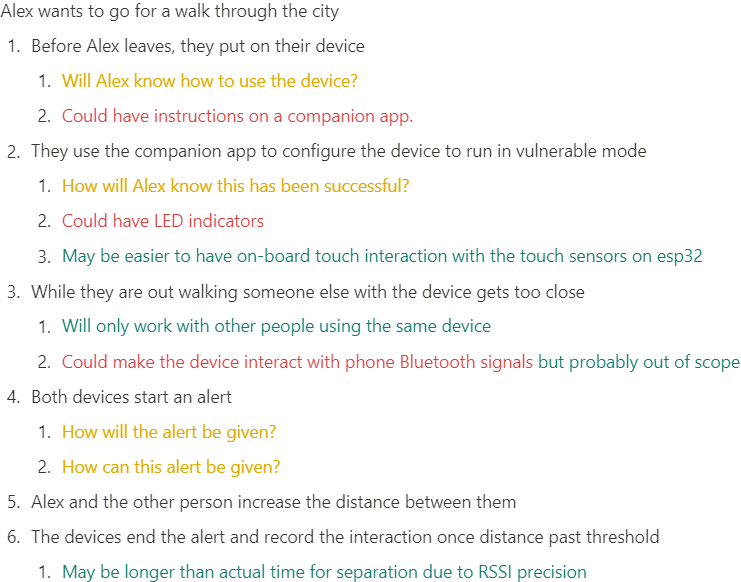
\includegraphics[width=1.0\linewidth]{images/user_story.png}

        \caption{ An example user scenario. }

        % use the notation fig:name to cross reference a figure
        \label{fig:alex_user_scenario}
    \end{figure}

\end{appendices}

%==================================================================================================================================
%   BIBLIOGRAPHY   

% The bibliography style is abbrvnat
% The bibliography always appears last, after the appendices.

\bibliographystyle{abbrvnat}

\bibliography{l4proj}

\end{document}
